% ===== Setup Page Layout =====
\documentclass{article}
\usepackage[a4paper, total={6in, 8in}]{geometry}
\usepackage{geometry}
 \geometry{
 a4paper,
 total={6in, 8in},
 left=35mm
 }
\usepackage{graphicx}

% ===== Setup Font =====
\usepackage[sfdefault,lf]{carlito}
\usepackage[T1]{fontenc}
\renewcommand*\oldstylenums[1]{\carlitoOsF #1}

% ==== Import Math Packages =====
\usepackage{amsmath, amssymb, amsthm}
\usepackage{mathtools}
\usepackage{pgfplots}
\pgfplotsset{compat=1.18}
\usetikzlibrary{decorations.pathreplacing,calligraphy}

% ==== Import Styling Packages =====
\usepackage{enumitem}
\usepackage[pages=some, placement=bottom]{background}
\usepackage{moresize}
\usepackage{relsize}
\usepackage{hyperref}
\hypersetup{colorlinks=true,allcolors=blue}
\usepackage{hypcap}
\usepackage{verbatim}

% ==== Import Drawing Packages =====
\usepackage{tikz}

% ==== Custom Declarations =====
\DeclarePairedDelimiter\abs{\lvert}{\rvert}
\DeclarePairedDelimiter\floor{\lfloor}{\rfloor}
\DeclarePairedDelimiter\cintervalc{[ }{] }
\DeclarePairedDelimiter\ointervalc{( }{] }
\DeclarePairedDelimiter\cintervalo{[ }{) }
\DeclarePairedDelimiter\ointervalo{( }{) }
\DeclarePairedDelimiter\set{\{ }{\} }
\DeclarePairedDelimiter\bracket{(}{)}
\newcommand{\drv}[2]{\frac{d}{d#1}\bracket*{#2}}
\newcommand{\drvL}[2]{D_{#1}\bracket*{#2}}
\newcommand{\ds}{\displaystyle}

% ===== Cover Setup =====
\backgroundsetup{
scale=1,
color=black,
opacity=1,
angle=0,
contents={%
  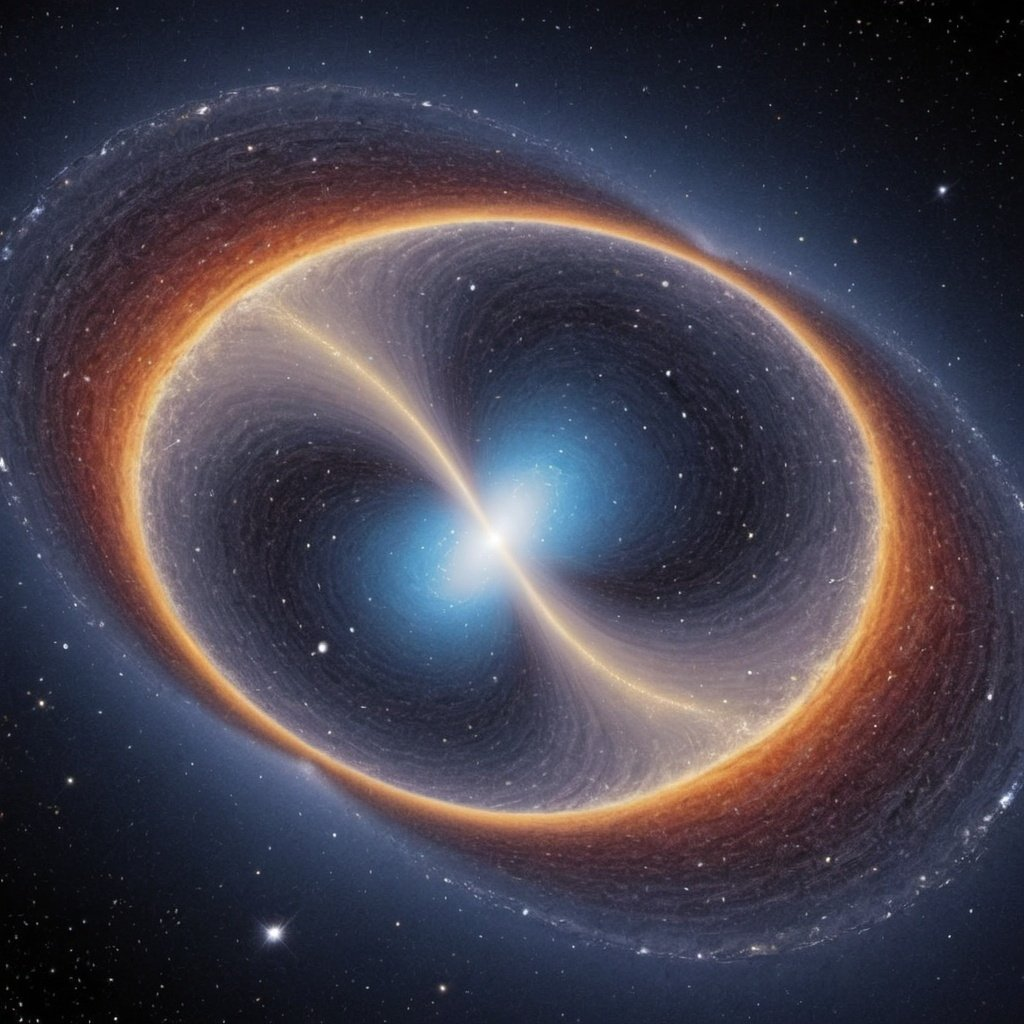
\includegraphics[width=\paperwidth,height=0.8\paperheight]{cover_kalkulus 1.png}
  }%
}

\title{Kalkulus 1}
\author{Fritz Adelbertus Sitindaon}
\date{July 2024}

\begin{document}
% ===== Cover =====
% \begin{center}
%     \textbf{\HUGE{KALKULUS 1}}

%     \vspace{0.5cm}
%     \textbf{\Large Kurikulum 2020}

%     \vspace{7cm}
%     \scalebox{15}{$\ds \lim_{x \to \infty}$}
% \end{center}
% \thispagestyle{empty}
% \newpage
% \tableofcontents

% \begin{flushright}
    \section*{\Large{Kuis 1}}
    \addcontentsline{toc}{section}{Kuis 1}
    \subsection*{Tahun 2020}
    \addcontentsline{toc}{subsection}{Kuis 1 - 2020}
\end{flushright}
\vspace{0.5cm}
\hrule height 2pt
\vspace{0.5cm}
%========= ========= ========= ========= ========= ========= ========= =========|||
\begin{center}
    \textbf{\large{MATERI}}
    \begin{enumerate}[leftmargin=*, label={\arabic*}.]
        \item Menyelesaikan pertidaksamaan yang melibatkan nilai mutlak.
        \item Mencari nilai limit kiri dan nilai limit kanan fungsi.
        \item Mencari nilai limit fungsi di tak hingga.
        \item Mencari nilai turunan fungsi menggunakan definisi.
        \item Menyelesaikan masalah turunan implisit.
        \item Menyelesaikan permasalahan laju yang berkaitan.
        \item Mencari nilai maksimum dan minimum fungsi.
    \end{enumerate}
\end{center}
\vspace{0.2cm}
\hrule height 1pt
\vspace{0.5cm}
\begin{center}
    \textbf{\large{SOAL}}
\end{center}
\begin{enumerate}[leftmargin=*, label={\arabic*}.]
\item Tentukanlah himpunan penyelesaian dari $\abs{2x-1} \geq 2\abs{x+1}$.
\item Hitunglah limit berikut (jika ada)!
    \begin{enumerate}[label={\alph*}.]
        \item $\ds \lim_{x\to -\infty} \frac{2x}{\abs{x}}$
        \item $\ds \lim_{x\to 5^{-}} \frac{x^{2}-3x-10}{x^{2}-10x+25}$
    \end{enumerate}
\item Diberikan fungsi 
$\ds
    f(x) = 
    \begin{cases}
        x+1, &\text{jika $x \geq 0$}\\
        x^{2}+1, &\text{jika $x < 0$}
    \end{cases}
$. Hitunglah $f'(0)$ (jika ada)!
\item Tentukanlah kemiringan garis singgung dari kurva $\cos (xy^{2})-\sin y = x$ 
di titik $(x,y) = (1,0)$.
\item Pada suatu empang yang tenang (tidak ada riak gelombang), dijatuhkan sebuah 
batu kecil, sehingga dihasilkan riak gelombang berbentuk lingkaran. Jari-jari 
riak-lingkaran tersebut bertambah dengan laju konstan 3 cm/detik. Seberapa cepat 
pertambahan \textbf{luas daerah} yang dijalani riak-lingkaran tersebut ketika 
jari-jari riak-lingkaran tersebut 10 cm?
\item Tentukanlah nilai maksimum dan nilai minimum fungsi $f(t)=t\sqrt{4-t^{2}}$ 
pada interval $I = \cintervalc*{-1,2}$
\end{enumerate}
\vspace{0.2cm}
\hrule height 1pt

\newpage
\begin{center}
    \textbf{\large{PEMBAHASAN}}
\end{center}
\begin{enumerate}[leftmargin=*, label={\arabic*}.]
\item Akan dicari himpunan penyelesaian dari $\abs{2x-1} \geq 2\abs{x+1}$.\\
Hanya ada 3 aturan dasar yang diperlukan untuk menyelesaikan pertidaksamaan.
\begin{enumerate}[label={\arabic*})]
    \item Jumlahkan kedua ruas dengan bilangan yang sama.
    \item Kalikan kedua ruas dengan bilangan positif yang sama.
    \item Kalikan kedua ruas dengan bilangan negatif yang sama dan 
    mengubah arah pertidaksamaannya.
\end{enumerate}
Pada soal ini kedua ruas melibatkan nilai mutlak. Untuk menyelesaikannya 
pertidaksamaan perlu diubah kebentuk yang tidak melibatkan nilai mutlak. 
Cara yang selalu bisa digunakan adalah dengan membagi kasus pada nilai $x$.

Perhatikan bahwa sesuai definisi nilai mutlak
\[
\abs{2x-1} = 
\begin{cases}
    2x-1, &\text{jika $2x-1 \geq 0$ atau $x \geq \frac{1}{2}$}\\
    -(2x-1), &\text{jika $2x-1 < 0$ atau $x < \frac{1}{2}$}
\end{cases}
\]
dan
\[
\abs{x+1} = 
\begin{cases}
    x+1, &\text{jika $x+1 \geq 0$ atau $x \geq -1$}\\
    -(x+1), &\text{jika $x+1 < 0$ atau $x < -1$}
\end{cases}
\]
Sehingga pertidaksamaan ini diselesaikan dengan membagi menjadi 3 kasus seperti 
yang terlihat pada garis bilangan di bawah ini.

\vspace{0.2cm}
\begin{tikzpicture}
\draw[stealth-stealth] (-6,0) node[below]{$-\infty$}--(5,0) node[below]{$\infty$};
\draw (-2,.1)--(-2,-.1) node[below=0.2em]{$-1$};
\draw (1,.1)--(1,-.1) node[below=0.2em]{$\frac{1}{2}$};
\node at (-7,1) {$\abs{2x-1}=$};
\node at (-7,.4) {$\abs{x+1}=$};

\node at (-4,1) {$-(2x-1)$};
\node at (-4,.4) {$-(x+1)$};

\node at (-.5,1) {$-(2x-1)$};
\node at (-.5,.4) {$x+1$};

\node at (3,1) {$-(2x-1)$};
\node at (3,.4) {$x+1$};
\end{tikzpicture}

\textbf{Kasus 1: $x < -1$}\\
Maka
\begin{align*}
    \abs{2x-1} \geq 2\abs{x+1} 
    \iff &-(2x-1) \geq 2(-(x+1)) 
    &\text{definisi nilai mutlak} \\
    \iff &1-2x \geq -2x-2
    &\text{penyederhanaan}\\
    \iff &1 \geq -2
    &\text{kedua ruas jumlahkan $2x$}
\end{align*}
Ini menandakan untuk semua nilai $x < -1$ pertidaksamaan akan ujungnya 
berbentuk $1 \geq -2$ yang selalu bernilai benar. Dengan kata lain, semua 
nilai $x < -1$ memenuhi pertidaksamaan.

\textbf{Kasus 2: $-1 \leq x < \frac{1}{2}$}\\
Maka
\begin{align*}
    \abs{2x-1} \geq 2\abs{x+1} 
    \iff &-(2x-1) \geq 2(x+1)
    &\text{definisi nilai mutlak} \\
    \iff &1-2x \geq 2x+2
    &\text{penyederhanaan}\\
    \iff &-4x \geq 1
    &\text{kedua ruas jumlahkan $-1-2x$}\\
    \iff &x \leq -\frac{1}{4}
    &\text{kedua ruas kalikan $-\frac{1}{4}$}
\end{align*}
Sehingga untuk kasus $-1 \leq x < \frac{1}{2}$ nilai $x$ yang memenuhi 
pertidaksamaan adalah $x \leq -\frac{1}{4}$. Dengan kata lain, nilai 
$-1 \leq x \leq -\frac{1}{4}$ memenuhi pertidaksamaan.

\textbf{Kasus 3: $x \geq \frac{1}{2}$}\\
Maka
\begin{align*}
    \abs{2x-1} \geq 2\abs{x+1} 
    \iff &2x-1 \geq 2(x+1)
    &\text{definisi nilai mutlak} \\
    \iff &2x-1 \geq 2x+2
    &\text{penyederhanaan}\\
    \iff &-1 \geq 2
    &\text{kedua ruas jumlahkan $-2x$}
\end{align*}
Ini menandakan untuk semua nilai $x \geq \frac{1}{2}$ pertidaksamaan 
akan ujungnya berbentuk $-1 \geq 2$ yang selalu bernilai salah.
Dengan kata lain, semua nilai $x \geq \frac{1}{2}$ tidak memenuhi 
pertidaksamaan.

Himpunan penyelesaiannya adalah gabungan semua nilai $x$ yang memenuhi 
pertidaksamaan. Sehingga himpunan tersebut adalah 
$\set*{x < -1 \cup -1 \leq x \leq -\frac{1}{4}}$ 
atau $\set*{x \in \mathbb{R} \mid x \leq -\frac{1}{4}}$
atau $\ointervalc*{-\infty,-\frac{1}{4}}$

$\therefore$ Himpunan penyelesaian dari $\abs{2x-1} \geq 2\abs{x+1}$
adalah $\set*{x \in \mathbb{R} \mid x \leq -\frac{1}{4}}$
atau $\ointervalc*{-\infty,-\frac{1}{4}}$

\vspace{0.1cm}
\textbf{Catatan:}\\
Salah satu cara untuk mengubah pertidaksamaan yang melibatkan nilai mutlak ke 
pertidaksamaan yang tidak adalah dengan menguadratkan kedua ruas. Soal ini 
dapat diselesaikan dengan cara tersebut tetapi tidak semua soal dapat 
diselesaikan dengan cara itu. Hal ini dikarenakan cara tersebut memiliki syarat 
yaitu kedua ruasnya harus bernilai positif.
\begin{center}
    \line(1,0){300}
\end{center}
\item Akan dicari limit dari soal yang diberikan (jika ada).
\begin{enumerate}[label={\alph*}.]
    \item Akan dicari limit dari 
    $\ds \lim_{x\to -\infty} \frac{2x}{\abs{x}}$
    \begin{align*}
        \lim_{x\to -\infty} \frac{2x}{\abs{x}} 
        &= \lim_{x\to -\infty} \frac{2x}{-x}
        &\text{definisi nilai mutlak $x < 0$ karena menuju $-\infty$}\\
        &= \lim_{x\to -\infty} \frac{2}{-1}
        &\text{kalikan $\frac{1/x}{1/x}$ (karena $x \neq 0$)}\\
        &= -2
        &\text{teorema utama limit}
    \end{align*}
    Sehingga nilai limit fungsi ini saat $x$ menuju $-\infty$ adalah $-2$

    $\therefore$ $\ds \lim_{x\to -\infty} \frac{2x}{\abs{x}} = -2$
\begin{center}
    \line(1,0){150}
\end{center}
    \item Akan dibuktikan 
    $\ds \lim_{x\to 5^{-}} \frac{x^{2}-3x-10}{x^{2}-10x+25}$ tidak ada.

    \begin{align*}
        \lim_{x\to 5^{-}} \frac{x^{2}-3x-10}{x^{2}-10x+25} 
        &= \lim_{x\to 5^{-}} \frac{(x-5)(x+2)}{(x-5)(x-5)}
        &\text{faktorisasi}\\
        &= \lim_{x\to 5^{-}} \frac{x+2}{x-5}
        &\text{kalikan $\frac{1/(x-5)}{1/(x-5)}$ (karena $x \neq 5$)}\\
        &= -\infty
        &\text{menuju bentuk $\frac{7}{0}$ dari kiri}
    \end{align*}
    Sehingga limitnya tidak ada.

    $\therefore$
    $\ds \lim_{x\to 5^{-}} \frac{x^{2}-3x-10}{x^{2}-10x+25} = -\infty$ 
    (tidak ada)
\end{enumerate}
\vspace{0.1cm}
\textbf{Catatan}:\\
Teorema-teorema limit yang sering digunakan ada pada Bab 1.3 buku rujukan \cite{valberg}
\begin{center}
    \line(1,0){300}
\end{center}
\item Akan dicari $f'(0)$ (jika ada) dengan.
\[
f(x) = 
\begin{cases}
    x+1, &\text{jika $x \geq 0$}\\
    x^{2}+1, &\text{jika $x < 0$}
\end{cases}
\]
Gunakan definisi limit dari turunan dimana
\[
f'(x) = \lim_{h\to 0} \frac{f(x+h)-f(x)}{h}
\]
Karena $f$ adalah fungsi \textit{pointwise} yang belum tentu memiliki turunan 
di $x=0$, akan dicari $f'(0)$ dengan mencari limit kiri dan limit kanan definisi 
limit turunannya.

Akan dicari $\ds \lim_{h\to 0^{-}} \frac{f(0+h)-f(0)}{h}$
\begin{align*}
    \lim_{h\to 0^{-}} \frac{f(0+h)-f(0)}{h}
    &= \lim_{h\to 0^{-}} \frac{f(h)-(0+1)}{h}
    &\text{subtitusi ke dalam fungsi}\\
    &= \lim_{h\to 0^{-}} \frac{h^{2}+1-1}{h}
    &\text{subtitusi ke dalam fungsi}\\
    &= \lim_{h\to 0^{-}} \frac{h^{2}}{h}
    &\text{sederhanakan}\\
    &= \lim_{h\to 0^{-}} h = 0
    &\text{kalikan $\frac{1/h}{1/h}$}
\end{align*}

Selanjutnya dicari $\ds \lim_{h\to 0^{+}} \frac{f(0+h)-f(0)}{h}$
\begin{align*}
    \lim_{h\to 0^{+}} \frac{f(0+h)-f(0)}{h}
    &= \lim_{h\to 0^{+}} \frac{f(h)-(0+1)}{h}
    &\text{subtitusi ke dalam fungsi}\\
    &= \lim_{h\to 0^{+}} \frac{h+1-1}{h}
    &\text{subtitusi ke dalam fungsi}\\
    &= \lim_{h\to 0^{+}} \frac{h}{h}
    &\text{sederhanakan}\\
    &= \lim_{h\to 0^{+}} 1 = 1
    &\text{kalikan $\frac{1/h}{1/h}$}
\end{align*}

Perhatikan bahwa
\[
\lim_{h\to 0^{-}} \frac{f(0+h)-f(0)}{h} = 0 
\neq 1 = \lim_{h\to 0^{+}} \frac{f(0+h)-f(0)}{h}
\]
sehingga $\ds \lim_{h\to 0} \frac{f(0+h)-f(0)}{h} = f'(0)$ tidak ada.

$\therefore$ $f'(0)$ tidak ada.
\begin{center}
    \line(1,0){300}
\end{center}
\item Akan dicari kemiringan garis singgung dari kurva $\cos (xy^{2})-\sin y = x$ di 
titik $(x,y) = (1,0)$.\\
Kemiringan garis singgung kurva dapat dicari dengan mencari nilai turunan dari kurva 
pada titik singgung. Pada soal ini titik tersebut adalah $(x,y) = (1,0)$, sehingga 
cukup mencari nilai turunan pertama kurva pada titik tersebut.\\
Gunakan metode untuk mencari turunan secara implisit dan aturan rantai.
\begin{align*}
    &\drv{x}{\cos (xy^{2})-\sin y} = \drv{x}{x}\\
    \iff &\drv{x}{\cos (xy^{2})} - \drv{x}{\sin y} = 1
    &\text{sifat linear turunan}\\
    \iff &\bracket*{-\sin(xy^{2})\drv{x}{xy^{2}}}
    -\bracket*{\cos y \drv{x}{y}} = 1
    &\text{aturan rantai}\\
    \iff &\bracket*{-\sin (xy^{2})\bracket*{y^{2}+xyy'}} 
    -\bracket*{\cos (y) y'} = 1
    &\text{aturan perkalian}
\end{align*}
Sekarang subtitusi $(x,y)=(1,0)$ untuk memperoleh nilai $y'$.
\begin{align*}
    &\bracket*{-\sin (xy^{2})\bracket*{y^{2}+xyy'}} - \bracket*{\cos (y) y'} = 1\\
    \iff &\bracket*{-\sin (1\cdot 0^{2})\bracket*{0^{2}+1\cdot 0\cdot y'}} - \bracket*{\cos (0) y'} = 1\\
    \iff &\bracket*{-\sin(0)(0)} - \bracket*{(1)y'} = 1\\
    \iff &-y' = 1 \iff y'=-1
\end{align*}
Diperoleh nilai turunan di titik $(x,y) = (1,0)$ adalah $-1$ sehingga kemiringan 
garis singgung kurva di titik tersebut adalah $-1$

$\therefore$ Kemiringan garis singgung kurva pada titik $(x,y) = (1,0)$ adalah $-1$.
\begin{center}
    \line(1,0){300}
\end{center}

\item Akan dicari cepat pertambahan luas daerah yang dijalani riak-lingkaran ketika 
jari-jarinya $10$ cm.\\
Misalkan $L=$ luas daerah riak-lingkaran dan $r=$ jari-jari riak-lingkaran.\\
Informasi yang diberikan soal adalah cepat pertambahan jari-jari riak-lingkaran yang 
konstan sehingga 
\[\drv{t}{r} = 3\]
Cepat pertambahan luas daerah adalah $\drvL{t}{L}$. Karena $L$ adalah luas 
riak-lingakaran maka 
\begin{center}
    $L = \pi r^{2}$ dan $\ds \drv{r}{L} = 2\pi r$
\end{center}
Dengan aturan rantai maka
\[
\drv{t}{L} = \drv{r}{L}\cdot\drv{t}{r} = 2\pi r \cdot 3 = 6\pi r
\]
Sehingga $\drvL{t}{L}$ saat $r=10$ adalah $60\pi$

$\therefore$ Cepat pertambahan luas daerah yang dijalani riak-lingkaran ketika 
jari-jarinya $10$ cm adalah $60\pi$ cm$^{2}$/detik.
\begin{center}
    \line(1,0){300}
\end{center}

\item 
Akan dicari nilai maksimum dan nilai minimum fungsi $f(t)=t\sqrt{4-t^{2}}$ pada 
interval $\cintervalc*{-1,2}$.\\
Carilah titik kritis dan uji nilai fungsi pada setiap titik tersebut untuk menemukan 
titik ekstrim.\\
Titik kritis terjadi pada
\begin{enumerate}[label={\arabic*})]
    \item Ujung interval
    \item Titik stasioner (saat $f'(c)=0$)
    \item Titik singular (saat $f'(c)$ tidak ada)
\end{enumerate}
Dengan demikian ujung interval $x=-1,2$ adalah titik kritis. Karena $f'(c)$ ada 
untuk semua $x$ pada interval $\cintervalc*{-1,2}$ maka tidak ada titik singular. Terakhir akan 
dicari titik stasioner.\\
Pertama akan dicari $f'(t)$ 
\begin{align*}
    f'(t) = \drv{t}{t\sqrt{4-t^{2}}} 
    &= \drv{t}{t\bracket*{4-t^{2}}^{1/2}}
    &\text{penyederhanaan}\\
    &= \bracket*{4-t^2}^{1/2}+t\bracket*{\frac{1}{2}\bracket*{4-t^{2}}^{-1/2}\cdot\drv{t}{4-t^{2}}}
    &\text{aturan perkalian \& rantai}\\
    &= \sqrt{4-t^{2}}+t\bracket*{\frac{1}{2\sqrt{4-t^{2}}}\cdot (-2t)}
    &\text{penyederhanaan}\\
    &= \frac{4-t^{2}-t^{2}}{\sqrt{4-t^{2}}}
    &\text{penyederhanaan}\\
    &= \frac{4-2t^{2}}{\sqrt{4-t^{2}}}
    &\text{penyederhanaan}
\end{align*}
Sehingga saat $f'(c)=0$ maka
\begin{align*}
    f'(c) &= \frac{4-2c^{2}}{\sqrt{4-c^{2}}} = 0\\
    \iff &4-2c^{2} = 0
    &\text{kedua ruas kalikan $\sqrt{4-c^{2}}$}\\
    \iff &-2c^{2} = -4
    &\text{kedua ruas ditambah $-4$}\\
    \iff &c^2 = 2
    &\text{kedua ruas kalikan $-\frac{1}{2}$}\\
\end{align*}
Nilai $c$ yang memenuhi adalah $c=-\sqrt{2}, \sqrt{2}$. Abaikan $-\sqrt{2}$ karena 
tidak terletak di interval $\cintervalc{-1,2}$ dan diperoleh titik stasioner 
$c = \sqrt{2}$.\\
Diperoleh tiga titik kritis $x = -1,\sqrt{2},2$.\\
Evaluasi fungsi pada ketiga titik tersebut diperoleh $f(-1) = -\sqrt{3}$, 
$f(\sqrt{2})=2$ dan $f(2) = 0$. Dengan demikian, titik maksimum terjadi pada 
$x = \sqrt{2}$ dan titik minimum terjadi pada $x = -1$

$\therefore$ Nilai maksimum dan nilai minimum fungsi $f(t)=t\sqrt{4-t^2}$ pada 
interval $\cintervalc{-1,2}$ adalah $2$ $\bracket*{\text{saat $x = \sqrt{2}$}}$ 
dan $-\sqrt{3}$ $\bracket*{\text{saat $x = -1$}}$.
\end{enumerate}
\begin{center}
    \line(1,0){300}
\end{center}
% \begin{flushright}
    \textbf{\Large{Kuis 1}}
    \subsection*{Tahun 2021}
    \addcontentsline{toc}{subsection}{Kuis 1 - 2021}
\end{flushright}
\vspace{0.5cm}
\hrule height 2pt
\vspace{0.5cm}
\begin{center}
    \textbf{\large{MATERI}}
    \begin{enumerate}[leftmargin=*, label={\arabic*}.]
        \item Menyelesaikan pertidaksamaan yang melibatkan nilai mutlak.
        \item Fungsi komposisi dan menentukan domainnya.
        \item Mencari nilai limit kiri dan nilai limit kanan fungsi.
        \item Menentukan kekontinuan fungsi pada suatu titik.
    \end{enumerate}
\end{center}
\vspace{0.2cm}
\hrule height 1pt
\vspace{0.5cm}
\begin{center}
    \textbf{\large{SOAL}}
\end{center}
\begin{enumerate}[leftmargin=*, label={\arabic*}.]
\item Diketahui 
$f(x) = \abs{x-2}$ dan 
$g(x) = x+1$.
\begin{enumerate}[label={\alph*}.]
    \item Tentukanlah nilai $x$ yang memenuhi $f(x) \leq g(x)$.
    \item Jika 
    $h(x) = \sqrt{g(x)}$, maka tentukanlah 
    $(f \circ h)(x)$ dan domain dari
    $(f \circ h)(x)$. Jelaskanlah jawaban anda!
\end{enumerate}
\item Misalkan
\[
    f(x) = 
    \begin{cases}
        2-x^{2}, &\text{jika $0 \leq x < 1$}\\
        \frac{5}{2}, &\text{jika $x = 1$}\\
        \abs{2-x}, &\text{jika $1 < x \leq 3$}\\
        \frac{a}{2x-3}, &\text{jika $3 < x \leq 5$}
    \end{cases}
\]
\begin{enumerate}[label={\alph*}.]
    \item Apakah fungsi $f$ kontinu di $x=1$? Jelaskanlah jawaban anda!
    \item Tentukan nilai $a$ sehingga $f$ kontinu di $x=3$. Jelaskanlah!
\end{enumerate}
\end{enumerate}
\vspace{0.2cm}
\hrule height 1pt
\vspace{0.5cm}

\begin{center}
    \textbf{\large{PEMBAHASAN}}
\end{center}
\begin{enumerate}[leftmargin=*, label={\arabic*}.]
\item
\begin{enumerate}[label={\alph*}.]
\item Akan dicari nilai $x$ yang memenuhi
$f(x) \leq g(x) \iff \abs{x-2} \leq x+1$.\\
Hanya ada 3 aturan dasar yang diperlukan untuk menyelesaikan pertidaksamaan.
\begin{enumerate}[label={\arabic*})]
    \item Jumlahkan kedua ruas dengan bilangan yang sama.
    \item Kalikan kedua ruas dengan bilangan positif yang sama.
    \item Kalikan kedua ruas dengan bilangan negatif yang sama dan 
    mengubah arah pertidaksamaannya.
\end{enumerate}
Pada soal ini ruas kiri melibatkan nilai mutlak. Untuk menyelesaikannya 
pertidaksamaan perlu diubah kebentuk yang tidak melibatkan nilai mutlak. 
Cara yang selalu bisa digunakan adalah dengan membagi kasus pada nilai $x$.
    
Perhatikan bahwa sesuai definisi nilai mutlak
\[
\abs{x-2} = 
\begin{cases}
    x-2, &\text{jika $x-2 \geq 0$ atau $x \geq 2$}\\
    -(x-2), &\text{jika $x-2 < 0$ atau $x < 2$}
\end{cases}
\]
Sehingga pertidaksamaan ini diselesaikan dengan membagi menjadi 2 kasus 
seperti yang terlihat pada garis bilangan di bawah ini.
    
\vspace{0.2cm}
\begin{tikzpicture}
\draw[stealth-stealth] (-6,0) node[below]{$-\infty$}--(5,0) node[below]{$\infty$};
\draw (0,.1)--(0,-.1) node[below=0.2em]{$2$};
\node at (-7,.4) {$\abs{x-2}=$};
    
\node at (-3,.4) {$-(x-2)$};
\node at (3,.4) {$x-2$};
\end{tikzpicture}
    
\textbf{Kasus 1: $x < 2$}\\
Maka
\begin{align*}
    \abs{x-2} \leq x+1
    \iff &-(x-2) \leq x+1 
    &\text{definisi nilai mutlak} \\
    \iff &2-x \leq x+1
    &\text{penyederhanaan}\\
    \iff &-2x \leq -1
    &\text{kedua ruas jumlahkan $-2-x$}\\
    \iff &x \geq \frac{1}{2}
    &\text{kedua ruas kalikan $-\frac{1}{2}$}
\end{align*}
Sehingga untuk kasus $x < 2$ nilai $x$ yang memenuhi pertidaksamaan adalah 
$x \geq \frac{1}{2}$. Dengan kata lain, nilai $-\frac{1}{2} \leq x < 2$ 
memenuhi pertidaksamaan.
    
\textbf{Kasus 2: $x \geq 2$}\\
Maka
\begin{align*}
    \abs{x-2} \leq x+1
    \iff &x-2 \leq x+1 
    &\text{definisi nilai mutlak} \\
    \iff &-2 \leq 1
    &\text{kedua ruas jumlahkan $-x$}
\end{align*}
Ini menandakan untuk semua nilai $x \geq 2$ pertidaksamaan akan ujungnya 
berbentuk $-2 \leq 1$ yang selalu bernilai benar. Dengan kata lain, semua 
nilai $x \geq 2$ memenuhi pertidaksamaan.
    
Semua nilai $x$ yang memenuhi $f(x) \leq g(x)$ adalah gabungan nilai $x$ 
dari kedua kasus. Sehingga nilai $x$ yang memenuhi adalah 
$\set*{\frac{1}{2} \leq x < 2 \cup x \geq 2}$ atau 
$\set*{x \in \mathbb{R} \mid x \geq \frac{1}{2}}$
atau $\cintervalo*{\frac{1}{2}, \infty}$
    
$\therefore$ Nilai $x$ yang memenuhi $f(x) \leq g(x)$ adalah
$\set*{x \in \mathbb{R} \mid x \geq \frac{1}{2}}$ atau
$\cintervalo*{\frac{1}{2}, \infty}$.
    
\vspace{0.1cm}
\textbf{Catatan:}\\
Salah satu cara untuk mengubah pertidaksamaan yang melibatkan nilai mutlak 
ke pertidaksamaan yang tidak adalah dengan menguadratkan kedua ruas. Soal 
ini \textbf{TIDAK} dapat diselesaikan dengan cara tersebut. Hal ini 
dikarenakan cara tersebut memiliki syarat yaitu kedua ruasnya harus bernilai 
positif. Pada kasus ini ruas kiri dapat bernilai negatif.
\begin{center}
    \line(1,0){150}
\end{center}
\item Akan dicari $(f \circ h)(x)$ dan domainnya.\\
Soal memberikan informasi bahwa $f(x) = \abs{x-2}$, $g(x) = x+1$ dan 
$h(x) = \sqrt{g(x)} = \sqrt{x+1}$.\\
Dengan definisi fungsi komposisi, maka
\[
    (f \circ h)(x) = f(h(x)) = f\bracket*{\sqrt{x+1}} = \abs*{\sqrt{x+1}-2}
\]
Domain dari komposisi $f \circ h$ adalah himpunan nilai $x$ dimana
\begin{enumerate}[label={\arabic*})]
    \item $x$ berada di dalam domain dari $h$
    \item $h(x)$ berada di dalam domain dari $f$
\end{enumerate}
Karena $h(x) = \sqrt{x+1}$ memiliki bentuk akar maka domain natural dari 
fungsi $h(x)$ adalah \\ $x+1 \geq 0 \iff x \geq -1$.
Selanjutnya karena range dari $h$ atau semua nilai $h(x)$ positif, maka
semua $h(x)$ berada di dalam domain dari $f$. Sehingga domain dari 
$f \circ h$ adalah $\set*{x \geq -1}$ atau $\cintervalo{-1,\infty}$
    
$\therefore$ $(f \circ h)(x) = \abs*{\sqrt{x+1} - 2}$ dengan domain 
$\set*{x \geq -1}$ atau $\cintervalo{-1,\infty}$ 
    
\vspace{0.1cm}
\textbf{Catatan:}\\
Cara mudah untuk mencari domainnya adalah mencari langsung domain 
$f \circ h$ dari $(f \circ h)(x)$ dan mengambil irisannya dengan 
domain dari $h$. (Lihat Kuis 1 2022 - 1b)
\begin{center}
    \line(1,0){300}
\end{center}
\end{enumerate}
\item
\begin{enumerate}[label={\alph*}.]
\item Akan dibuktikan $f$ tidak kontinu di $x=1$.\\
Tiga syarat untuk membuktikan $f$ kontinu di $x=1$ adalah
\begin{enumerate}[label={\arabic*}.]
    \item $\lim_{x\to 1} f(x)$ ada.
    \item $f(1)$ ada.
    \item $\lim_{x\to 1} f(x) = f(1)$
\end{enumerate}
Membuktikan tidak berlaku maka menunjukan salah satu syarat tersebut tidak
terpenuhi.\\
$\lim_{x\to 1} f(x)$ ada karena limit kanan dan limit kiri ada dan bernilai sama.
\begin{align*}
    \lim_{x\to 1^{-}} f(x) 
    &= \lim_{x\to 1^{-}} 2-x^{2}
    &\text{definisi fungsi $f$}\\
    &= 2-1^{2} = 1
    &\text{teorema subtitusi}\\
    \lim_{x\to 1^{+}} f(x) 
    &= \lim_{x\to 1^{+}} \abs{2-x}
    &\text{definisi fungsi $f$}\\
    &= \abs{2-1} = 1
    &\text{teorema subtitusi}
\end{align*}
$f(1)$ ada karena sesuai definisi soal bahwa $f(1) = \frac{5}{2}$.\\
Syarat ketiga tidak terpenuhi karena
\[
    \lim_{x\to 1} f(x) = 1 \neq \frac{5}{2} = f(1)
\].
Sehingga $f$ tidak kontinu di $x=1$ karena tidak memenuhi syarat ketiga

$\therefore$ $f$ tidak kontinu di $x=1$ karena $\lim_{x\to 1} f(x) \neq f(1)$
\begin{center}
    \line(1,0){150}
\end{center}
\item Akan dicari nilai $a$ sehingga $f$ kontinu di $x=3$.\\
Sama seperti sebelumnya, tiga syarat untuk membuktikan $f$ kontinu di
$x=3$ adalah:
\begin{enumerate}[label={\arabic*}.]
    \item $\lim_{x\to 3} f(x)$ ada.
    \item $f(3)$ ada.
    \item $\lim_{x\to 3} f(x) = f(3)$
\end{enumerate}
Mulai dengan menentukan $a$ sehingga limit fungsi di $x=3$ ada. Hal ini 
dapat dilakukan dengan menyamakan limit kanan dan limit kiri.
\begin{align*}
    \lim_{x\to 3^{-}} f(x) 
    &= \lim_{x\to 3^{-}} \abs{2-x}
    &\text{definisi fungsi $f$}\\
    &= \abs{2-3} = 1
    &\text{teorema subtitusi}\\
    \lim_{x\to 3^{+}} f(x) 
    &= \lim_{x\to 3^{+}} \frac{a}{2x-3}
    &\text{definisi fungsi $f$}\\
    &= \frac{a}{6-3} = \frac{a}{3}
    &\text{teorema subtitusi}
\end{align*}
Pilih $a = 3$ sehingga
\[
    \lim_{x\to 3^{+}} f(x) = \frac{a}{3} = \frac{3}{3} = 1 = \lim_{x\to 3^{-}} f(x) 
\]
Syarat pertama terpenuhi yaitu $\lim_{x\to 3} f(x) = 1$ ada.\\
Syarat kedua terpenuhi karena dari definisi fungsi $f(3) = \abs{2-3} = 1$.\\
Syarat ketiga juga terpenuhi karena $\lim_{x\to 3} f(x) = 1 = f(3)$.
Sehingga dengan memilih $a=3$ fungsi $f$ kontinu di $x=3$.

$\therefore$ Nilai $a$ sehingga $f$ kontinu di $x=3$ adalah $a=3$.
\end{enumerate}
\end{enumerate}
\begin{center}
    \line(1,0){300}
\end{center}
% \begin{flushright}
    \textbf{\Large{Kuis 1}}
    \subsection*{Tahun 2022}
    \addcontentsline{toc}{subsection}{Kuis 1 - 2022}
\end{flushright}
\vspace{0.5cm}
\hrule height 2pt
\vspace{0.5cm}
\begin{center}
    \textbf{\large{MATERI}}
    \begin{enumerate}[leftmargin=*, label={\arabic*}.]
        \item Menyelesaikan pertidaksamaan yang melibatkan bentuk rasional.
        \item Fungsi komposisi dan menentukan domainnya.
        \item Mencari nilai limit dari fungsi.
        \item Menentukan kekontinuan fungsi pada suatu titik.
    \end{enumerate}
\end{center}
\vspace{0.2cm}
\hrule height 1pt
\vspace{0.5cm}
\begin{center}
    \textbf{\large{SOAL}}
\end{center}
\begin{enumerate}[leftmargin=*, label={\arabic*}.]
\item Diketahui $f(x) = x$ dan $\ds g(x) = \frac{x}{x+4}$.
\begin{enumerate}[label={\alph*}.]
    \item Tentukanlah nilai $x$ yang memenuhi $f(x) \leq g(x)$.
    \item Jika $h(x) = \sqrt{f(x)}$, maka tentukanlah $(h \circ g)(x)$ 
    dan domain dari $(h \circ g)(x)$. Jelaskanlah jawaban anda!
\end{enumerate}
\item Misalkan diberikan fungsi berikut ini: 
$\ds k(x) = \frac{x^{2}-4}{x^{2}-5x+6}$
\begin{enumerate}[label={\alph*}.]
    \item Tentukan diskontinuitas dari fungsi $k$ dan jelaskan mengapa fungsi
    itu gagal kontinu pada titik-titik tersebut.
    \item Tentukan titik-titik yang dapat dihapus dan yang tidak dapat dihapus
    diskontinuitasnya.
\end{enumerate}
\end{enumerate}
\vspace{0.2cm}
\hrule height 1pt
\vspace{0.5cm}

\begin{center}
    \textbf{\large{PEMBAHASAN}}
\end{center}
\begin{enumerate}[leftmargin=*, label={\arabic*}.]
\item
\begin{enumerate}[label={\alph*}.]
\item Akan dicari nilai $x$ yang memenuhi
$\ds f(x) \leq g(x) \iff x \leq \frac{x}{x+4}$.

\vspace{0.1cm}
Hanya ada 3 aturan dasar yang diperlukan untuk menyelesaikan pertidaksamaan.
\begin{enumerate}[label={\arabic*})]
    \item Jumlahkan kedua ruas dengan bilangan yang sama.
    \item Kalikan kedua ruas dengan bilangan positif yang sama.
    \item Kalikan kedua ruas dengan bilangan negatif yang sama dan 
    mengubah arah pertidaksamaannya.
\end{enumerate}
Soal ini melibatkan bentuk rasional. Lakukan pembagian kasus sehingga kedua
ruas dapat dikalikan $(x+4)$
    
\textbf{Kasus 1: }$x+4 > 0$ atau $x>-4$\\
Maka $x+4$ adalah bilangan \textbf{positif} dan
\begin{align*}
    x \leq \frac{x}{x+4}
    \iff &x(x+4) \leq x
    &\text{kedua ruas kalikan $(x+4)$}\\
    \iff &x^{2}+4x \leq x
    &\text{penyederhanaan}
\end{align*}
Bagi menjadi subkasus lagi sehingga kedua ruas dapat dibagi $x$\\
\textbf{Subkasus 1.1: }$x>-4$ dan $x>0$\\
Maka $x$ adalah bilangan \textbf{positif} dan saat dilanjutkan
\begin{align*}
    x^{2}+4x \leq x
    \iff &x+4 \leq 1
    &\text{kedua ruas kalikan $\frac{1}{x}$}\\
    \iff &x \leq -3
    &\text{kedua ruas jumlahkan $-4$}
\end{align*}
Didapat nilai $x$ yang memenuhi adalah $x\leq -3$. Ini berkontradiksi dengan
kasus ini yang dimana $x > 0$. Sehingga tidak ada nilai $x$ yang memenuhi
pada subkasus ini. \\
\textbf{Subkasus 1.2: }$x>-4$ dan $x<0$\\
Maka $-4 < x < 0$ dan $x$ adalah bilangan \textbf{negatif}, saat dilanjutkan
\begin{align*}
    x^{2}+4x \leq x
    \iff &x+4 \geq 1
    &\text{kedua ruas kalikan $\frac{1}{x}$}\\
    \iff &x \geq -3
    &\text{kedua ruas jumlahkan $-4$}
\end{align*}
Didapat nilai $x$ yang memenuhi adalah $x \geq -3$. Syarat pada subkasus
ini adalah $-4 < x < 0$ sehingga nilai $x$ yang memenuhi pada subkasus ini
adalah $-3 \leq x < 0$ \\
\textbf{Subkasus 1.3: }$x>-4$ dan $x=0$\\
Maka pertidaksamaan menjadi $0 \leq 0$ yang bernilai benar. Nilai $x=0$
memenuhi pertidaksamaan pada subkasus ini.

\textbf{Kasus 2: }$x+4 < 0$ atau $x < -4$\\
Maka $x+4$ dan $x$ adalah bilangan \textbf{negatif} dan
\begin{align*}
    x \leq \frac{x}{x+4}
    \iff &x(x+4) \geq x
    &\text{kedua ruas kalikan $(x+4)$}\\
    \iff &x^{2}+4x \geq x
    &\text{penyederhanaan}\\
    \iff &x+4 \leq 1
    &\text{kedua ruas kalikan $\frac{1}{x}$}\\
    \iff &x \leq -3
    &\text{kedua ruas jumlahkan $-4$}
\end{align*}
Didapat nilai $x$ yang memenuhi adalah $x \leq -3$. Syarat pada kasus
ini adalah $x < -4$ sehingga nilai $x$ yang memenuhi pada kasus ini
adalah $x < -4$ \\
    
Semua nilai $x$ yang memenuhi $f(x) \leq g(x)$ adalah gabungan nilai $x$ 
dari semua kasus. Sehingga nilai $x$ yang memenuhi adalah 
$\set*{-3 \leq x < 0 \cup x = 0 \cup x < -4}$ atau 
$\set*{x \in \mathbb{R} \mid x \geq x < -4 \cup -3 \leq x \leq 0}$
atau $\ointervalc*{-\infty, -4} \cup \cintervalc*{-3,0}$
    
$\therefore$ Nilai $x$ yang memenuhi $f(x) \leq g(x)$ adalah
$\set*{x \in \mathbb{R} \mid x \geq x < -4 \cup -3 \leq x \leq 0}$\\
atau $\ointervalc*{-\infty, -4} \cup \cintervalc*{-3,0}$
    
\vspace{0.1cm}
\textbf{Catatan:}\\
Ini merupakan cara yang menerapkan konsep dasar dari penyelesaian
pertidaksamaan. Untuk pembahasan selanjutnya akan digunakan cara yang 
lebih cepat.
\begin{center}
    \line(1,0){150}
\end{center}
\item Akan dicari $(h \circ g)(x)$ dan domainnya.\\
Soal memberikan informasi bahwa $f(x) = x$, $g(x) = \frac{x}{x+4}$ 
dan $h(x) = \sqrt{f(x)} = \sqrt{x}$.\\
Dengan definisi fungsi komposisi, maka
\[
    (h \circ g)(x) = h(g(x)) = h\bracket*{\frac{x}{x+4}} 
    = \sqrt{\frac{x}{x+4}}
\]
Untuk menemukan domainnya, carilah irisan dari domain  
$\ds \sqrt{\frac{x}{x+4}}$ dan $g(x)=\ds\frac{x}{x+4}$\\
Pertama karena terdapat bilangan rasional, maka penyebutnya tidak boleh
nol, sehingga $x+4 \neq 0$ atau $x\neq-4$. Lalu karena ada bentuk akar, 
maka nilai didalam akarnya harus nonnegatif.
\begin{align*}
    \frac{x}{x+4} \geq 0.
\end{align*}
Maka $x=0$ dan $x+4=0$ adalah titik belok.

\vspace{0.2cm}
\begin{tikzpicture}
\draw[stealth-stealth] (-6,0) node[below]{$-\infty$}--(5,0) node[below]{$\infty$};
\draw (-6,1) --(-2,1);
\draw (2,1) --(5,1);
\draw (-2,1)--(-2,-.1) node[below=0.2em]{$-4$};
\draw (2,1)--(2,-.1) node[below=0.2em]{$0$};
    
\node at (3.5,.5) {$+$};
\node at (-4,.5) {$+$};
\node at (0,.5) {$-$};
\node [draw, shape = circle, fill = black, minimum size = 0.1cm, inner sep=0pt] at (2,0){};
\node [draw, shape = circle, fill = white, minimum size = 0.1cm, inner sep=0pt] at (-2,0){};
\end{tikzpicture}\\
Sehingga domainnya adalah $x < 4 \cup x \geq 0$.

Lalu domain dari $g$ adalah semua nilai $x \neq -4$
Sehingga domain dari $(h \circ g)(x)$ adalah
\[
\set*{x \in R \mid x < 4 \cup x \geq 0} \cap \set*{x \in R \mid x \neq 4} 
= \set*{x \in R \mid x < 4 \cup x \geq 0}
\]

$\therefore$ $\ds (h \circ g)(x) = \sqrt{\frac{x}{x+4}}$ dengan domain 
$\set*{x \in R \mid x < 4 \cup x \geq 0}$ 
\begin{center}
    \line(1,0){300}
\end{center}
\end{enumerate}
\item
\begin{enumerate}[label={\alph*}.]
\item Akan dicari titik dikontinuitas fungsi $k$\\
Tiga syarat untuk membuktikan $k$ kontinu di $x=c$ adalah
\begin{enumerate}[label={\arabic*}.]
    \item $\lim_{x\to c} f(x)$ ada.
    \item $f(c)$ ada.
    \item $\lim_{x\to c} f(x) = f(c)$
\end{enumerate}
$k$ adalah fungsi yang memiliki bentuk rasional. Diskontinuitas terjadi saat 
di titik dimana penyebut bernilai nol, karena fungsi $k$ tidak terdefinisi 
di titik itu dan syarat kedua kontinuitas tidak terpenuhi.
Jika titik $c$ adalah pembuat nol penyebut maka
\begin{align*}
    c^{2} - 5c + 6 = 0
    \iff &(c-2)(c-3) = 0
    &\text{faktorisasi}
\end{align*}
sehingga titik dikontinuitas $k$ adalah saat $x=2$ dan $x=3$ karena syarat kedua 
tidak terpenuhi.

$\therefore$ $k$ diskontinu di $x=2$ dan $x=3$ karena $k(x)$ tidak ada pada 
$x$ tersebut.
\begin{center}
    \line(1,0){150}
\end{center}
\item Hasil dari soal sebelumnya akan diuji. Diskontinuitas dapat dihapus jika limit 
fungsi pada titik tersebut ada. Sehingga pendefinisian ulang fungsi dapat membuat 
syarat kedua dan ketiga kontinuitas terpenuhi.

Akan dicari limit $k$ di titik $x=2$ dan $x=3$.\\
Untuk $x=2$
\begin{align*}
    \lim_{x \to 2} \frac{x^{2}-4}{x^{2}-5x+6}
    &= \lim_{x \to 2} \frac{(x-2)(x+2)}{(x-2)(x-3)}
    &\text{faktorisasi}\\
    &= \lim_{x \to 2} \frac{x+2}{x-3}
    &\text{kalikan $\frac{1/(x-2)}{1/(x-2)}$ (karena $x \neq 2$)}\\
    &= \frac{2+2}{2-3} = -4
    &\text{teorema subtitusi}
\end{align*}
Karena nilai limitnya ada maka dikontinuitas di $x=2$ dapat dihapus.\\
Untuk $x=3$\\
Limitny tidak ada, karena saat $x$ mendekati $3$ maka $x-2$ mendekati $1$, 
$x+2$ mendekati $5$ dan $x-3$ mendekati 0. Sehingga limit dari fungsi ini 
saat $x$ mendekati $3$ adalah bentuk yang mendekati $\frac{5}{0}$. Dari kanan 
bentuk ini mendekati $\infty$ dan dari kiri mendekati $-\infty$ sehingga limit 
kiri dan limit kanannya tidak ada.\\
Karena nilai limitnya tidak ada maka diskontinuitas di $x=3$ tidak dapat dihapus.

$\therefore$ Titik yang dikontinuitasnya dapat dihapus adalah $x=2$ dan yang tidak 
dapat dihapus adalah $x=3$.
\begin{center}
    \line(1,0){300}
\end{center}
\end{enumerate}
\end{enumerate}

% \begin{flushright}
    \textbf{\Large{Kuis 1}}
    \subsection*{Tahun 2023}
    \addcontentsline{toc}{subsection}{Kuis 1 - 2023}
\end{flushright}
\vspace{0.5cm}
\hrule height 2pt
\vspace{0.5cm}
\begin{center}
    \textbf{\large{MATERI}}
    \begin{enumerate}[leftmargin=*, label={\arabic*}.]
        \item Menyelesaikan pertidaksamaan yang melibatkan nilai mutlak.
        \item Fungsi komposisi dan menentukan domainnya.
        \item Mencari nilai limit kiri dan nilai limit kanan fungsi.
        \item Menentukan kekontinuan fungsi pada suatu titik.
    \end{enumerate}
\end{center}
\vspace{0.2cm}
\hrule height 1pt
\vspace{0.5cm}
\begin{center}
    \textbf{\large{SOAL}}
\end{center}
\begin{enumerate}[leftmargin=*, label={\arabic*}.]
\item Misalkan $f(x) = x^{2}-x$ dan $g(x)=\abs{x-1}$.
\begin{enumerate}[label={\alph*}.]
    \item Tentukanlah nilai $x$ yang memenuhi $f(x) > g(x)$.
    \item Jika $\ds h(x) = \frac{g(x)}{f(x)}$, maka tentukanlah 
    domain dari $h(x)$. Jelaskanlah jawaban anda!
\end{enumerate}
\item Misalkan
\[
    f(x) =
    \begin{cases}
        c^{2}x^{2}, &{x < 2},\\
        (1-c)x, &{x \geq 2}.
    \end{cases}
\]
Tentukan nilai $c$ agar $f$ kontinu di setiap bilangan real $x$.
\end{enumerate}
\vspace{0.2cm}
\hrule height 1pt
\vspace{0.5cm}

\begin{center}
    \textbf{\large{PEMBAHASAN}}
\end{center}
\begin{enumerate}[leftmargin=*, label={\arabic*}.]
\item
\begin{enumerate}[label={\alph*}.]
\item Akan dicari nilai $x$ yang memenuhi
$f(x) > g(x) \iff x^{2}-x > \abs{x-1}$.

\vspace{0.1cm}
Hanya ada 3 aturan dasar yang diperlukan untuk menyelesaikan pertidaksamaan.
\begin{enumerate}[label={\arabic*})]
    \item Jumlahkan kedua ruas dengan bilangan yang sama.
    \item Kalikan kedua ruas dengan bilangan positif yang sama.
    \item Kalikan kedua ruas dengan bilangan negatif yang sama dan 
    mengubah arah pertidaksamaannya.
\end{enumerate}
Pada soal ini ruas kanan melibatkan nilai mutlak. Untuk menyelesaikannya 
pertidaksamaan perlu diubah kebentuk yang tidak melibatkan nilai mutlak. Cara yang 
selalu bisa digunakan adalah dengan membagi kasus pada nilai $x$.
    
Perhatikan bahwa sesuai definisi nilai mutlak
\[
\abs{x-1} = 
\begin{cases}
    x-1, &\text{jika $x-1 \geq 0$ atau $x \geq 1$}\\
    -(x-1), &\text{jika $x-1 < 0$ atau $x < 1$}
\end{cases}
\]
Sehingga pertidaksamaan ini diselesaikan dengan membagi menjadi 2 kasus 
seperti yang terlihat pada garis bilangan di bawah ini.
    
\vspace{0.2cm}
\begin{tikzpicture}
\draw[stealth-stealth] (-6,0) node[below]{$-\infty$}--(5,0) node[below]{$\infty$};
\draw (0,.1)--(0,-.1) node[below=0.2em]{$1$};
\node at (-7,.4) {$\abs{x-1}=$};
    
\node at (-3,.4) {$-(x-1)$};
\node at (3,.4) {$x-1$};
\end{tikzpicture}
    
\textbf{Kasus 1: $x < 1$}\\
Maka
\begin{align*}
    x^{2}-x > \abs{x-1}
    \iff &x^{2}-x > -(x-1)
    &\text{definisi nilai mutlak} \\
    \iff &x^{2}-x > 1-x
    &\text{penyederhanaan}\\
    \iff &x^{2} - 1 > 0
    &\text{kedua ruas jumlahkan $x-1$}\\
    \iff &(x+1)(x-1) > 0
    &\text{faktorisasi}
\end{align*}
Maka $x=1$ dan $x=-1$ adalah titik stasioner.

\begin{center}
\begin{tikzpicture}
    \draw[stealth-stealth] (-6,0) node[below]{$-\infty$}--(5,0) node[below]{$\infty$};
    \draw (-6,1) --(-2,1);
    \draw (2,1) --(5,1);
    \draw (-2,1)--(-2,-.1) node[below=0.2em]{$-1$};
    \draw (2,1)--(2,-.1) node[below=0.2em]{$1$};
            
    \node at (3.5,.5) {$+$};
    \node at (-4,.5) {$+$};
    \node at (0,.5) {$-$};
    \node [draw, shape = circle, fill = white, minimum size = 0.1cm, inner sep=0pt] at (2,0){};
    \node [draw, shape = circle, fill = white, minimum size = 0.1cm, inner sep=0pt] at (-2,0){};
    \end{tikzpicture}
\end{center}
Nilai yang memenuhi adalah $x < -1$ atau $x > 1$.
Karena syarat kasus ini adalah $x < 1$ maka nilai $x$ yang memenuhi adalah
$x < -1$.

\textbf{Kasus 2: $x \geq 1$}\\
Maka
\begin{align*}
    x^{2}-x > \abs{x-1}
    \iff &x^{2}-x > x-1
    &\text{definisi nilai mutlak} \\
    \iff &x^{2} -2x + 1> 0
    &\text{kedua ruas jumlahkan $-x+1$}\\
    \iff &(x-1)(x-1) > 0
    &\text{faktorisasi}
\end{align*}
Maka $x=-1$ dan $x=-1$ adalah titik stasioner.

\begin{center}
\begin{tikzpicture}
    \draw[stealth-stealth] (-6,0) node[below]{$-\infty$}--(5,0) node[below]{$\infty$};
    \draw (-6,1) --(0,1);
    \draw (0,1) --(5,1);
    \draw (0,1)--(0,-.1) node[below=0.2em]{$1$};
            
    \node at (3.5,.5) {$+$};
    \node at (-4,.5) {$+$};
    \node [draw, shape = circle, fill = white, minimum size = 0.1cm, inner sep=0pt] at (0,0){};
    \node [draw, shape = circle, fill = white, minimum size = 0.1cm, inner sep=0pt] at (0,0.1){};
    \end{tikzpicture}
\end{center}
Nilai yang memenuhi adalah $x \neq 1$.
Karena syarat kasus ini adalah $x \geq 1$ maka nilai $x$ yang memenuhi adalah
$x > 1$.
    
Semua nilai $x$ yang memenuhi $f(x) > g(x)$ adalah gabungan nilai $x$ 
dari kedua kasus. Sehingga nilai $x$ yang memenuhi adalah 
$\set*{x \in \mathbb{R} \mid x < -1 \cup x > 1}$
atau $\ointervalc*{-\infty, -1} \cup \cintervalo*{1, \infty}$
    
$\therefore$ Nilai $x$ yang memenuhi $f(x) > g(x)$ adalah
$\set*{x \in \mathbb{R} \mid x < -1 \cup x > 1}$
atau $\ointervalc*{-\infty, -1} \cup \cintervalo*{1, \infty}$

\begin{center}
    \line(1,0){150}
\end{center}
\item Akan dicari domain dari $\ds h(x) = \frac{g(x)}{f(x)}$.\\
Dari definisi tersebut ini adalah fungsi komposisi dengan 
\[
    h(x) = \frac{g(x)}{f(x)} = \frac{\abs{x-1}}{x^{2}-x}
\]
Sehingga domainnya adalah irisan dari domain $f$, $g$, dan 
$\ds \frac{\abs{x-1}}{x^{2}-x}$.\\
Domain dari $f$ dan $g$ adalah $\mathbb{R}$, sehingga cukup mencari 
domain dari $\ds \frac{\abs{x-1}}{x^{2}-x}$. Karena melibatkan 
bentuk rasional maka penyebut tidak boleh nol. Sehingga
\begin{align*}
    x^{2}-x \neq 0 \iff &x(x-1)\neq 0
    &\text{faktorisasi}
\end{align*}
Sehingga $x \neq 1$ dan $x \neq 0$. \\Domain dari 
$\ds \frac{\abs{x-1}}{x^{2}-x}$ adalah 
$\set*{x \in \mathbb{R} \mid x \neq 1, x\neq 0}$.\\ Irisan dari ketiga domain
$\mathbb{R}$, $\mathbb{R}$, dan $\set*{x \in \mathbb{R} \mid x \neq 1, x\neq 0}$ 
adalah $\set*{x \in \mathbb{R} \mid x \neq 1, x\neq 0}$.\\
Dengan demikian domain dari $h$ adalah 
$\set*{x \in \mathbb{R} \mid x \neq 1, x\neq 0}$.

$\therefore$ Domain dari fungsi $h$ adalah 
$\set*{x \in \mathbb{R} \mid x \neq 1, x\neq 0}$

\begin{center}
    \line(1,0){300}
\end{center}
\end{enumerate}
\item
\begin{enumerate}[label={\alph*}.]
\item \[
f(x) = 
\begin{cases}
    c^{2}x^{2}, &{x < 2},\\
    (1-c)x, &{x \geq 2}.
\end{cases}
\]
Akan dicari nilai $c$ agar fungsi $f$ kontinu di setiap bilangan real.\\
Bagian pertama dari fungsi \textit{pointwise} ini adalah bentuk kuadratik, 
dan yang kedua adalah bentuk linear. Keduanya kontinu di setiap bilangan real. 
Sehingga titik yang mungkin menyebabkan diskontinuitas hanya di $x=2$.

Tiga syarat untuk membuktikan $f$ kontinu di $x=2$ adalah
\begin{enumerate}[label={\arabic*}.]
    \item $\lim_{x\to 2} f(x)$ ada.
    \item $f(2)$ ada.
    \item $\lim_{x\to 2} f(x) = f(2)$
\end{enumerate}
Karena fungsi $f$ diharapkan kontinu di setiap bilangan real, diasumsikan $f$ 
juga memenuhi ketiga syarat diatas. Maka dari syarat pertama $\lim_{x\to 2} f(x)$ 
ada. Jika limitnya ada maka limit kanan dan kirinya ada dan 
\[
\lim_{x\to 2^{-}} f(x) = \lim_{x\to 2^{+}} f(x)
\]
sehingga
\begin{align*}
    \lim_{x\to 2^{-}} f(x) = \lim_{x\to 2^{+}} f(x)
    \iff &\lim_{x\to 2^{-}} c^{2}x^{2} = \lim_{x\to 2^{+}} (1-c)x\\
    \iff &c^{2}2^{2} = (1-c)2\\
    \iff &2c^{2} = 1-c\\
    \iff &2c^{2}+c-1 = 0\\
    \iff &(2c-1)(c+1) = 0
\end{align*}
Dari syarat pertama maka haruslah $c=-1$ atau $c=\frac{1}{2}$\\
Misalkan $c=-1$ maka limit saat $x$ menuju 2 adalah 4 (Subtitusi ke limit kiri dan 
kanannya). Akan dipastikan kedua syarat lainnya berlaku. Syarat kedua berlaku 
dengan $f(2) = (1-(-1))2 = 4$. Syarat ketiga juga berlaku karena 
$\lim_{x\to 2} f(x) = 4 = f(2)$.\\
Misalkan $c=\frac{1}{2}$ maka limit saat $x$ menuju 2 adalah 1 (Subtitusi ke limit 
kiri dan kanannya). Akan dipastikan kedua syarat lainnya berlaku. Syarat kedua berlaku 
dengan
\[
    f(2) = \bracket*{1-\frac{1}{2}}2 = 1
\] 
dan syarat ketiga juga berlaku Karena
\[
    \lim_{x\to 2} f(x) = 1 = f(2)
\] 
Sehingga kedua nilai $c=-1$ dan $c=\frac{1}{2}$ akan membuat fungsi $f$ 
kontinu di setiap bilangan real.

$\therefore$ Nilai $c$ agar fungsi $f$ kontinu di setiap bilangan real adalah $c=-1$ 
dan $c=\frac{1}{2}$
\begin{center}
    \line(1,0){300}
\end{center}
\end{enumerate}
\end{enumerate}

% \newpage
\begin{flushright}
    \section*{\Large{Ujian Tengah Semester}}
    \addcontentsline{toc}{section}{Ujian Tengah Semester (UTS)}
    \subsection*{Tahun 2020}
    \addcontentsline{toc}{subsection}{UTS - 2020}
\end{flushright}
\vspace{0.5cm}
\hrule height 2pt
\vspace{0.5cm}
\begin{center}
    \textbf{\large{MATERI}}
    \begin{enumerate}[leftmargin=*, label={\arabic*}.]
        \item Memahami konsep nilai mutlak
        \item Menyelesaikan pertidaksamaan yang melibatkan nilai mutlak.
        \item Mensketsa grafik fungsi.
        \item Fungsi komposisi dan menentukan domain dan rangenya.
        \item Mencari nilai limit kiri dan nilai limit kanan fungsi.
        \item Mencari nilai limit fungsi di tak hingga.
        \item Menentukan kekontinuan fungsi pada suatu titik.
        \item Menyelesaikan masalah turunan implisit.
        \item Menyelesaikan permasalahan maksimum dan minimum.
    \end{enumerate}
\end{center}
\vspace{0.2cm}
\hrule height 1pt
\vspace{0.5cm}
\begin{center}
    \textbf{\large{SOAL}}
\end{center}
\begin{enumerate}[leftmargin=*, label={\arabic*}.]
\item 
\begin{enumerate}[label={\alph*}.]
    \item Tentukanlah himpunan penyelesaian dari 
    $\ds \abs*{\frac{x}{x+2}} \geq x$.
    \item Jika terdapat persamaan yang menyatakan bahwa $|-a| = a$, 
    maka untuk nilai-nilai $a$ berapakah persamaan tersebut menjadi 
    benar atau salah?
\end{enumerate}
\item Diberikan fungsi 1 variabel bernilai real $f(x)$ dan $g(x)$ sebagai berikut:
\begin{center}
    $\ds f(x) = 
    \begin{cases}
        \abs{x+1}, &\text{jika $x < 1$}\\
        -x^{2}+4, &\text{jika $x \geq 1$}
    \end{cases}$ dan $\ds g(x) = \frac{1}{x}$
\end{center}
\begin{enumerate}[label={\alph*}.]
    \item Sketsalah grafik fungsi $f(x)$ dan $g(x)$ tanpa menggunakan bantuan
    \textit{software}.    
    \item Tentukanlah $(g \circ f)(x)$ sedemikian sehingga rumus fungsinya tidak 
    memuat nilai mutlak, kemudian tentukanlah domain dan range dari $(g \circ f)(x)$.
    \item Apakah 
    $\ds \floor*{(g \circ f)(0.5)} = \brk*{\frac{g \circ f}{g}}(0.5)$? 
    Jelaskanlah jawaban Anda!
\end{enumerate}
\item Diberikan fungsi $f\colon \mathbb{R} \to \mathbb{R}$ dengan $f(1)=f(-1)=1$ 
dan $\ds f(x) = \frac{x^{2}-x}{x^{2}-1}$ untuk $x$ lainnya.
\begin{enumerate}[label={\alph*}.]
    \item Hitunglah $\ds \lim_{x \to \infty} f(x)$ (jika ada)! 
    \item Hitunglah $\ds \lim_{x \to -\infty} f(x)$ (jika ada)! 
    \item Hitunglah $\ds \lim_{x \to 1} f(x)$ (jika ada)! 
    \item Hitunglah $\ds \lim_{x \to -1} f(x)$ (jika ada)!
    \item Apakah fungsi $f$ kontinu di titik $x=1$? Jelaskanlah! Jika $f$ tidak 
    kontinu di titik tersebut, apakah ketidakkontinuannya dapat diperbaiki? 
    Jelaskanlah! 
    \item Apakah fungsi $f$ kontinu di titik $x=-1$? Jelaskanlah! Jika $f$ tidak 
    kontinu di titik tersebut, apakah ketidakkontinuannya dapat diperbaiki? 
    Jelaskanlah! 
\end{enumerate}
\item 
\begin{enumerate}[label={\alph*}.]
    \item Tentukanlah persamaan garis singgung yang menyinggung kurva \\
    $xy^{2}+y(x^{2}+1)^{2} = y^{2}+x$ di titik $(0,1)$.
    \item Tentukanlah turunan kedua dari fungsi implisit di soal sebelumnya 
    pada titik $(0,1)$.
\end{enumerate}
\item Tentukanlah panjang dan lebar suatu persegi panjang yang bisa dimasukkan 
kedalam elips dengan persamaan $\ds \frac{x^{2}}{a}+\frac{y^{2}}{b}=1$ 
sedemikian sehingga luas persegi panjang tersebut maksimum.
\end{enumerate}
\vspace{0.2cm}
\hrule height 1pt
\vspace{0.5cm}
\begin{center}
    \textbf{\large{PEMBAHASAN}}
\end{center}
\begin{enumerate}[leftmargin=*, label={\arabic*}.]
\item
\begin{enumerate}[label={\alph*}.]
    \item Akan dicari himpunan penyelesaian dari 
    $\ds \abs*{\frac{x}{x+2}} \geq x$.\\
    Hanya ada 3 aturan dasar yang diperlukan untuk menyelesaikan pertidaksamaan.
    \begin{enumerate}[label={\arabic*})]
        \item Jumlahkan kedua ruas dengan bilangan yang sama.
        \item Kalikan kedua ruas dengan bilangan positif yang sama.
        \item Kalikan kedua ruas dengan bilangan negatif yang sama dan 
        mengubah arah pertidaksamaannya.
    \end{enumerate}
    Pada soal ini ruas kiri melibatkan nilai mutlak. Untuk menyelesaikannya 
    pertidaksamaan perlu diubah kebentuk yang tidak melibatkan nilai mutlak. 
    Cara yang selalu bisa digunakan adalah dengan membagi kasus pada nilai $x$.
        
    Perhatikan bahwa sesuai definisi nilai mutlak
    \[
    \abs*{\frac{x}{x+2}} = 
    \begin{cases}
        \frac{x}{x+2}, &\text{jika $\frac{x}{x+2} \geq 0$ atau $x < -2 \cup x \geq 0$ $^{*1}$}\\
        -\frac{x}{x+2}, &\text{jika $\frac{x}{x+2} < 0$ atau $-2 < x < 0$ $^{*2}$}
    \end{cases}
    \]
    (*1) $\frac{x}{x+2} \geq 0$ dapat disederhanakan dengan menyelesaikan 
    pertidaksamaannya. \\Titik stasioner pertidaksamaan ini adalah $x= 0$ dan $x=-2$.
    \begin{center}
    \begin{tikzpicture}
        \draw[stealth-stealth] (-5,0) node[below]{$-\infty$}--(5,0) node[below]{$\infty$};
        \draw (-5,1) --(-2,1);
        \draw (2,1) --(5,1);
        \draw (-2,1)--(-2,-.1) node[below=0.2em]{$-2$};
        \draw (2,1)--(2,-.1) node[below=0.2em]{$0$};
                
        \node at (3.5,.5) {$+$};
        \node at (-4,.5) {$+$};
        \node at (0,.5) {$-$};
        \node [draw, shape = circle, fill = black, minimum size = 0.1cm, inner sep=0pt] at (2,0){};
        \node [draw, shape = circle, fill = white, minimum size = 0.1cm, inner sep=0pt] at (-2,0){};
    \end{tikzpicture}
    \end{center}
    Sehingga
    \[
        \frac{x}{x+2} \geq 0 \iff x < -2 \cup x \geq 0
    \]
    (*2) $\frac{x}{x+2} < 0$ dengan gambaran garis bilangan yang sama seperti sebelumnya
    \[
        \frac{x}{x+2} < 0 \iff -2 < x < 0
    \]
    Sehingga pertidaksamaan ini diselesaikan dengan membagi menjadi 2 kasus seperti 
yang terlihat pada garis bilangan di bawah ini.

\vspace{0.2cm}
\begin{tikzpicture}
\draw[stealth-stealth] (-6,0) node[below]{$-\infty$}--(5,0) node[below]{$\infty$};
\draw (-2,.1)--(-2,-.1) node[below=0.2em]{$-2$};
\draw (1,.1)--(1,-.1) node[below=0.2em]{$0$};
\node at (-7,.7) {$\ds \abs*{\frac{x}{x+2}}=$};

\node at (-4,.7) {$\ds \frac{x}{x+2}$};
\node at (-.5,.7) {$\ds -\frac{x}{x+2}$};
\node at (3,.7) {$\ds \frac{x}{x+2}$};
\end{tikzpicture}

\textbf{Kasus 1: $x < -2 \cup x \geq 0$}\\
Maka
\begin{align*}
    \abs*{\frac{x}{x+2}} \geq x
    \iff &\frac{x}{x+2} \geq x
    &\text{definisi nilai mutlak} \\
    \iff &\frac{x}{x+2} -x \geq 0
    &\text{kedua ruas jumlahkan $-x$}\\
    \iff &\frac{-x^{2}-x}{x+2} \geq 0
    &\text{penyederhanaan}\\
    \iff &\frac{x^{2}+x}{x+2} \leq 0
    &\text{kedua ruas kalikan $-1$}\\
    \iff &\frac{x(x+1)}{x+2} \leq 0
    &\text{faktorisasi}\\
\end{align*}
Titik stasioner pertidaksamaan ini adalah $x=-2$, $x=-1$, dan $x=0$.
\begin{center}
    \begin{tikzpicture}
        \draw[stealth-stealth] (-5,0) node[below]{$-\infty$}--(5,0) node[below]{$\infty$};
        \draw (-5,1) --(-2,1);
        \draw (0,1) --(2,1);
        \draw (-2,1)--(-2,-.1) node[below=0.2em]{$-2$};
        \draw (0,1)--(0,-.1) node[below=0.2em]{$-1$};
        \draw (2,1)--(2,-.1) node[below=0.2em]{$0$};
                
        \node at (3.5,.5) {$+$};
        \node at (-4,.5) {$-$};
        \node at (1,.5) {$-$};
        \node at (-1,.5) {$+$};
        \node [draw, shape = circle, fill = black, minimum size = 0.1cm, inner sep=0pt] at (2,0){};
        \node [draw, shape = circle, fill = black, minimum size = 0.1cm, inner sep=0pt] at (0,0){};
        \node [draw, shape = circle, fill = white, minimum size = 0.1cm, inner sep=0pt] at (-2,0){};
    \end{tikzpicture}
\end{center}
Sehingga nilai $x$ yang memenuhi pertidaksamaan adalah $x < -2 \cup -1 \leq x \leq 0$. Ambil 
irisannya dengan syarat pada kasus ini maka himpunan penyelesaian pada kasus ini adalah 
\\$\set{x < -2 \, \cup \, x = 0}$. 

\textbf{Kasus 2: $-2 < x < 0$}\\
Maka
\begin{align*}
    \abs*{\frac{x}{x+2}} \geq x
    \iff &-\frac{x}{x+2} \geq x
    &\text{definisi nilai mutlak} \\
    \iff &-\frac{x}{x+2} -x \geq 0
    &\text{kedua ruas jumlahkan $-x$}\\
    \iff &\frac{-x^{2}-3x}{x+2} \geq 0
    &\text{penyederhanaan}\\
    \iff &\frac{x^{2}+3x}{x+2} \leq 0
    &\text{kedua ruas kalikan $-1$}\\
    \iff &\frac{x(x+3)}{x+2} \leq 0
    &\text{faktorisasi}\\
\end{align*}
Titik stasioner pertidaksamaan ini adalah $x=-3$, $x=-2$, dan $x=0$.
\begin{center}
    \begin{tikzpicture}
        \draw[stealth-stealth] (-5,0) node[below]{$-\infty$}--(5,0) node[below]{$\infty$};
        \draw (-5,1) --(-3,1);
        \draw (-1,1) --(3,1);
        \draw (-1,1)--(-1,-.1) node[below=0.2em]{$-2$};
        \draw (-3,1)--(-3,-.1) node[below=0.2em]{$-3$};
        \draw (3,1)--(3,-.1) node[below=0.2em]{$0$};
                
        \node at (4,.5) {$+$};
        \node at (-4,.5) {$-$};
        \node at (1,.5) {$-$};
        \node at (-2,.5) {$+$};
        \node [draw, shape = circle, fill = black, minimum size = 0.1cm, inner sep=0pt] at (3,0){};
        \node [draw, shape = circle, fill = black, minimum size = 0.1cm, inner sep=0pt] at (-3,0){};
        \node [draw, shape = circle, fill = white, minimum size = 0.1cm, inner sep=0pt] at (-1,0){};
    \end{tikzpicture}
\end{center}
Sehingga nilai $x$ yang memenuhi pertidaksamaan adalah $x \leq -3 \cup -2 < x \leq 0$. Ambil 
irisannya dengan syarat pada kasus ini maka himpunan penyelesaian pada kasus ini adalah 
\\$\set{-2 < x < 0}$. 

Himpunan penyelesaiannya adalah gabungan semua nilai $x$ yang memenuhi pertidaksamaan. 
Sehingga himpunan tersebut adalah 
$\set*{x < -2 \cup x = 0 \cup -2 < x < 0}$ 
atau \\
$\set*{x \in \mathbb{R} \mid x < -2 \cup -2 < x \leq 0}$
atau
$\oic*{-\infty,0} \cap \set{x \in \mathbb{R} \mid x \neq 2}$

$\therefore$ Himpunan penyelesaian dari 
$\ds \abs*{\frac{x}{x+2}} \geq x$ adalah 
$\set*{x \in \mathbb{R} \mid x < -2 \cup -2 < x \leq 0}$
atau \\
$\oic*{-\infty,0} \cap \set{x \in \mathbb{R} \mid x \neq 2}$

\vspace{0.1cm}
\textbf{Catatan:}\\
Salah satu cara untuk mengubah pertidaksamaan yang melibatkan nilai mutlak ke 
pertidaksamaan yang tidak adalah dengan menguadratkan kedua ruas. Soal ini \textbf{TIDAK} 
dapat diselesaikan dengan cara tersebut. Hal ini dikarenakan cara tersebut memiliki syarat 
yaitu kedua ruasnya harus bernilai positif.
\begin{center}
    \line(1,0){150}
\end{center}
\item Diberikan persamaan $\abs{-a} = a$, akan dicari interval dimana nilai $a$ menghasilkan
persamaan yang benar dan persamaan yang salah.\\
Menggunakan definisi nilai mutlak maka
\[
    \abs{-a} = 
    \begin{cases}
        -a, &-a \geq 0 \iff a \leq 0\\
        -(-a), &-a < 0 \iff a > 0
    \end{cases}
\]
\textbf{Kasus 1: $a \leq 0$}\\
Maka $\abs{-a} = a \iff -a = a$. Persamaan ini benar hanya saat $a = 0$.\\
Sehingga untuk $a < 0$ persamaan ini menjadi salah sedangkan $a = 0$ menjadi benar.\\
\textbf{Kasus 2: $a > 0$}\\
Maka $\abs{-a} = a \iff -(-a) = a \iff a = a$. Persamaan ini 
selalu benar. Sehingga untuk $a > 0$, persamaan ini menjadi benar.

$\therefore$ Persamaan ini bernilai benar untuk $a \geq 0$ dan bernilai salah untuk $a < 0$.
\end{enumerate}
\begin{center}
    \line(1,0){300}
\end{center}
\item Diberikan
\begin{center}
    $\ds f(x) = 
    \begin{cases}
        \abs{x+1}, &\text{jika $x < 1$}\\
        -x^{2}+4, &\text{jika $x \geq 1$}
    \end{cases}$ dan $\ds g(x) = \frac{1}{x}$
\end{center}
\begin{enumerate}[label={\alph*}.]
    \item Akan disketsa grafik fungsi $f$ dan $g$\\
    3 tahap sketsa grafik adalah:
    \begin{enumerate}[label={\arabic*})]
        \item Cari beberapa titik koordinat $(x,f(x))$.
        \item Plot titik pada bidang
        \item Hubungkan titik-titik menjadi sebuah kurva
    \end{enumerate}
    Karena $f$ adalah fungsi \textit{pointwise} maka dibagi menjadi 2 bagian, saat
    $x < 1$ dan $x \geq 1$.\\
    Untuk $x < 1$, $f(x) = |x+1|$ cari titik dimana $|x+1|=0$ dan dua titik di kiri 
    dan kanannya. Berikut hasilnya dalam tabel.
    \begin{center}
    \begin{tabular}{|c|c|c|c|}\hline
        $x$ & $-2$ & $-1$ & $0$ \\ \hline
        $f(x)$ & $1$ & $0$ & $1$ \\ \hline
    \end{tabular}
    \end{center}
    Untuk $x \geq 1$, karena fungsinya kuadratik, cari tiga titik berbeda (sifat interpolasi).
    Berikut hasilnya dalam tabel.
    \begin{center}
    \begin{tabular}{|c|c|c|c|}\hline
        $x$ & $1$ & $2$ & $3$ \\ \hline
        $f(x)$ & $3$ & $0$ & $-5$ \\ \hline
    \end{tabular}
    \end{center}

Plot keenam titik tersebut dalam bidang kartesian dan hubungkan sehingga diperolah grafik 
seperti berikut.
\begin{center}
\begin{tikzpicture}[>=stealth]
\begin{axis}[
    xmin=-4,xmax=4,
    ymin=-6,ymax=4,
    axis x line=middle,
    axis y line=middle,
    axis line style=<->,
    xlabel={$x$},
    ylabel={$f(x)$},
    ]
    \addplot[no marks,blue, <-] expression[domain=-3:1,samples=100]{abs(x+1)} 
        node[pos=0,anchor=south west]{$\abs{x+1}$};
    \addplot[no marks,blue, ->] expression[domain=1:3.1,samples=100]{-x^2+4} 
        node[pos=0.25,anchor=south west]{$-x^{2}+4$}; 
    \node [draw, shape = circle, fill = white, minimum size = 0.1cm, inner sep=0pt] at (1,2){};
    \node [draw, shape = circle, fill = black, minimum size = 0.1cm, inner sep=0pt] at (1,3){};
    \node [draw, shape = circle, fill = black, minimum size = 0.1cm, inner sep=0pt] at (2,0){};
    \node [draw, shape = circle, fill = black, minimum size = 0.1cm, inner sep=0pt] at (3,-5){};
    \node [draw, shape = circle, fill = black, minimum size = 0.1cm, inner sep=0pt] at (-2,1){};
    \node [draw, shape = circle, fill = black, minimum size = 0.1cm, inner sep=0pt] at (-1,0){};
    \node [draw, shape = circle, fill = black, minimum size = 0.1cm, inner sep=0pt] at (0,1){};
\end{axis}
\end{tikzpicture}
\end{center}
Untuk $g(x) = \frac{1}{x}$ adalah fungsi spesial yang sangat disarankan untuk diingat bentuk grafiknya. 
Cara yang sama dapat dilakukan (Uji tiga titik $x < 0$ dan tiga titik $x > 0$)
\begin{center}
\begin{tikzpicture}[>=stealth]
\begin{axis}[
    xmin=-5,xmax=5,
    ymin=-5,ymax=5,
    axis x line=middle,
    axis y line=middle,
    axis line style=<->,
    xlabel={$x$},
    ylabel={$g(x)$},
    ]
    \addplot[no marks,blue, <-] expression[domain=-5:-0.01,samples=50]{1/x} 
        node[pos=0,anchor=south west]{};
    \addplot[no marks,blue, ->] expression[domain=0.01:5,samples=50]{1/x} 
        node[pos=0,anchor=south west]{};
    \node [draw, shape = circle, fill = black, minimum size = 0.1cm, inner sep=0pt] at (0.5,2){};
    \node [draw, shape = circle, fill = black, minimum size = 0.1cm, inner sep=0pt] at (1,1){};
    \node [draw, shape = circle, fill = black, minimum size = 0.1cm, inner sep=0pt] at (2,0.5){};
    \node at (1.25,2) {\scalebox{0.75}{$(0.5,2)$}};
    \node at (1.75,1.2) {\scalebox{0.75}{$(1,1)$}};
    \node at (3,0.8) {\scalebox{0.75}{$(2,0.5)$}};
    \node [draw, shape = circle, fill = black, minimum size = 0.1cm, inner sep=0pt] at (-0.5,-2){};
    \node [draw, shape = circle, fill = black, minimum size = 0.1cm, inner sep=0pt] at (-1,-1){};
    \node [draw, shape = circle, fill = black, minimum size = 0.1cm, inner sep=0pt] at (-2,-0.5){};
    \node at (-2,-2) {\scalebox{0.75}{$(-0.5,-2)$}};
    \node at (-2,-1.2) {\scalebox{0.75}{$(-1,-1)$}};
    \node at (-2,0.25) {\scalebox{0.75}{$(-2,-0.5)$}};
\end{axis}
\end{tikzpicture}
\end{center}
$\therefore$ Telah disketsa grafik $f$ dan $g$ seperti gambar diatas.
\begin{center}
    \line(1,0){150}
\end{center}
\item Akan dicari $(g \circ f)(x)$ sehingga fungsinya tidak memuat nilai mutlak.\\
Nilai mutlak berasal dari fungsi $f$ ketika $x < 1$, nilai mutlak ini dapat dihilangkan 
dengan menjabarkan kasus dari nilai mutlak. Sesuai definisi nilai mutlak:
\[
    \abs{x+1} =
    \begin{cases}
    x+1, &x+1 \geq 0 \iff x \geq -1,\\
    -(x+1), &x+1 < 0 \iff x < -1
    \end{cases}
\]
dengan demikian fungsi $f$ dapat diubah menjadi
\[
    f(x) = 
    \begin{cases}
        -(x+1), & x < -1,\\
        x+1, &-1 \leq x < 1,\\
        -x^{2}+4, &x \geq 1.
    \end{cases}
\]
sehingga fungsi komposisi $(g \circ f)(x)$ adalah
\[
    (g\circ f)(x) = g(f(x)) = 
    \begin{cases}
        \frac{1}{-(x+1)}, & x < -1,\\
        \frac{1}{x+1}, &-1 \leq x < 1 \quad ^*(x \neq -1),\\
        \frac{1}{-x^{2}+4}, &x \geq 1 \quad ^*(x \neq 2).
    \end{cases}
\]
Selanjutnya akan dicari domain dari $(g \circ f)(x)$. \\
Domain dari $(g \circ f)(x)$ adalah irisan dari domain $f$ dengan domain dari setiap kasus 
pada fungsi \textit{pointwise} $(g \circ f)(x)$. Fungsi $f$ hanya 
melibatkan bentuk linear dan kuadratik, sehingga domainnya adalah $\mathbb{R}$.\\

Domain dari $\ds \frac{1}{-(x+1)}$.

Karena melibatkan bentuk rasional maka $-(x+1) \neq 0 \iff x \neq -1$. Karena 
syarat kasus ini $x < -1$ maka domainnya adalah $x < -1$.

Domain dari $\ds \frac{1}{x+1}$.

Karena melibatkan bentuk rasional maka $x+1 \neq 0 \iff x \neq -1$. Karena 
syarat kasus ini $-1 \leq x < 1$, maka domainnya adalah $-1 < x < 1$.

Domain dari $\ds \frac{1}{-x^{2}+4}$.

Karena melibatkan bentuk rasional maka $-x^{2}+4 \neq 0 \iff x \neq -2,2$.\\
Karena syarat kasus ini $x \geq 1$, maka domainnya adalah $x \geq 1 \cap x \neq 2$.\\
Bila digabung maka domain dari $(g \circ f)(x)$ adalah 
$\set*{x \in \mathbb{R} \mid x \neq -1, x\neq 2}$ \\

Terakhir akan dicari range dari $(g \circ f)(x)$.

Dari kasus $\ds \frac{1}{-x^{2}+4}$ 
karena $\ds \lim_{x\to 2^{+}} (g \circ f)(x) = -\infty$ dan 
$\ds \lim_{x\to \infty} (g \circ f)(x) = 0$ maka 
$\oio{-\infty,0}$ adalah bagian dari range $g \circ f$.\\
Dari kasus $\ds \frac{1}{-(x+1)}$ 
karena $\ds \lim_{x\to -1^{-}} (g \circ f)(x) = \infty$ dan 
$\ds \lim_{x\to -\infty} (g \circ f)(x) = 0$ maka 
$\oio{0,\infty}$ adalah bagian dari range $g \circ f$.

Sehingga range dari $g \circ f$ sudah mencakup semua bilangan real kecuali $0$.
Dan karena $g \circ f$ berbentuk rasional dengan penyebut bernilai satu maka $0$ 
tidak bisa menjadi hasil dari $g \circ f$.

Dengan demikian range dari $(g \circ f)(x)$ adalah $\oio{-\infty,\infty} \cap x \neq 0$ 
atau $\set{y \in \mathbb{R} \mid y \neq 0}$.

Berikut grafik pendukung.

\begin{center}
\begin{tikzpicture}[>=stealth]
\begin{axis}[
    xmin=-5,xmax=5,
    ymin=-5,ymax=5,
    axis x line=middle,
    axis y line=middle,
    axis line style=<->,
    xlabel={$x$},
    ylabel={$(g \circ f)(x)$},
    ]
    \addplot[no marks,blue, <-] expression[domain=-5:1,samples=99]{1/abs(x+1)} 
        node[pos=0,anchor=south west]{};
    \addplot[no marks,blue, -] expression[domain=1:1.99,samples=20]{1/(-x^2+4)} 
        node[pos=0,anchor=south west]{};
    \addplot[no marks,blue, ->] expression[domain=2.01:5,samples=80]{1/(-x^2+4)} 
        node[pos=0,anchor=south west]{};
    \node [draw, shape = circle, fill =  white, minimum size = 0.08cm, inner sep=0pt] at (1,0.5){};
    \node [draw, shape = circle, fill = blue, minimum size = 0.08cm, inner sep=0pt] at (1,1/3){};  
\end{axis}
\end{tikzpicture}
\end{center}

$\therefore$ 
\[
    (g\circ f)(x) = g(f(x)) = 
    \begin{cases}
        \frac{1}{-(x+1)}, & x < -1,\\
        \frac{1}{x+1}, &-1 < x < 1 \\
        \frac{1}{-x^{2}+4}, &x > 1,\,x \neq 2.
    \end{cases}
\]
dengan domain $\set*{x \in \mathbb{R} \mid x \neq -1, x\neq 2}$ dan range
$\set{y \in \mathbb{R} \mid y \neq 0}$.
\begin{center}
    \line(1,0){150}
\end{center}
\item Akan diuji kebenaran dari 
$\ds \floor*{(g \circ f)(0.5)} = \brk*{\frac{g \circ f}{g}}(0.5)$.

Evaluasi nilai $\floor*{(g \circ f)(0.5)}$.
\begin{align*}
    \floor*{(g \circ f)(0.5)}
    &= \floor*{g(f(0.5))}
    &\text{definisi komposisi} \\
    &= \floor*{g(abs{0.5+1})} 
    &\text{evaluasi fungsi $f$} \\
    &= \floor*{g(1.5)}
    &\text{penyederhanaan}\\
    &=\floor*{\frac{1}{1.5}}
    &\text{evaluasi fungsi $g$}\\
    &=0 
    &\text{evaluasi $floor$}
\end{align*}

Evaluasi nilai $\ds \brk*{\frac{g \circ f}{g}}(0.5)$
\begin{align*}
    \brk*{\frac{g \circ f}{g}}(0.5) &= \frac{(g\circ f)(0.5)}{g(0.5)}\\
    &= \frac{g(f(0.5))}{g(0.5)} 
    &\text{definisi komposisi}\\
    &= \frac{g(\abs{0.5+1})}{g(0.5)}
    &\text{evaluasi fungsi $f$} \\
    &= \frac{g(1.5)}{g(0.5)} 
    &\text{penyederhanaan}\\
    &= \frac{1/1.5}{1/0.5}
    &\text{evaluasi fungsi $g$}\\
    &=\frac{0.5}{1.5} = \frac{1}{3}
    &\text{penyederhanaan}
\end{align*}
Diperoleh 
\[
    \floor*{(g \circ f)(0.5)} = 0 \neq \frac{1}{3} = \brk*{\frac{g \circ f}{g}}(0.5)
\]

$\therefore$ 
$\ds \floor*{(g \circ f)(0.5)} \neq \brk*{\frac{g \circ f}{g}}(0.5)$
\end{enumerate}
\begin{center}
    \line(1,0){300}
\end{center}
\item Diberikan fungsi $f\colon \mathbb{R} \to \mathbb{R}$ dengan $f(1)=f(-1)=1$ 
dan $\ds f(x) = \frac{x^{2}-x}{x^{2}-1}$ untuk $x$ lainnya.
\begin{enumerate}[label={\alph*}.]
    \item Akan dicari $\ds \lim_{x \to \infty} f(x)$ (jika ada).
    \begin{align*}
        \lim_{x \to \infty} f(x) 
        &= \lim_{x \to \infty} \frac{x^{2}-x}{x^{2}-1}
        &\text{karena fungsi mendekati $\infty$}\\
        &= \lim_{x \to \infty} \frac{1-\frac{1}{x}}{1-\frac{1}{x^{2}}}
        &\text{kalikan $\frac{1/x^{2}}{1/x^{2}}$ (karena $x \neq 0$)}\\
        &=\frac{\lim_{x \to \infty} 1 - \lim_{x \to \infty} \frac{1}{x}}
        {\lim_{x \to \infty} 1 - \lim_{x \to \infty}\frac{1}{x^{2}}}
        &\text{teorema utama limit}\\
        &= \frac{\lim_{x \to \infty} 1 - 0}{\lim_{x \to \infty} 1 - 0}
        &\text{karena $\lim_{x\to\infty}\frac{1}{x} = \lim_{x\to\infty}\frac{1}{x^{2}} = 0$}\\
        &= \frac{1}{1} = 1
        &\text{teorema utama limit}
    \end{align*} 
    $\therefore$ $\ds \lim_{x \to \infty} f(x)$ ada dan 
    $\ds \lim_{x \to \infty} f(x) = 1$
\begin{center}
    \line(1,0){150}
\end{center}
    \item Akan dicari $\ds \lim_{x \to -\infty} f(x)$ (jika ada).
    \begin{align*}
        \lim_{x \to -\infty} f(x) 
        &= \lim_{x \to -\infty} \frac{x^{2}-x}{x^{2}-1}
        &\text{karena fungsi mendekati $-\infty$}\\
        &= \lim_{x \to -\infty} \frac{1-\frac{1}{x}}{1-\frac{1}{x^{2}}}
        &\text{kalikan $\frac{1/x^{2}}{1/x^{2}}$ (karena $x \neq 0$)}\\
        &=\frac{\lim_{x \to -\infty} 1 - \lim_{x \to -\infty} \frac{1}{x}}
        {\lim_{x \to- \infty} 1 - \lim_{x \to -\infty}\frac{1}{x^{2}}}
        &\text{teorema utama limit}\\
        &= \frac{\lim_{x \to -\infty} 1 - 0}{\lim_{x \to -\infty} 1 - 0}
        &\text{karena $\lim_{x\to -\infty}\frac{1}{x} = \lim_{x\to -\infty}\frac{1}{x^{2}} = 0$}\\
        &= \frac{1}{1} = 1
        &\text{teorema utama limit}
    \end{align*} 
    $\therefore$ $\ds \lim_{x \to -\infty} f(x)$ ada dan 
    $\ds \lim_{x \to -\infty} f(x) = 1$
\begin{center}
\line(1,0){150}
\end{center}
    \item Akan dicari $\ds \lim_{x \to 1} f(x)$ (jika ada).
    \begin{align*}
        \lim_{x \to 1} f(x) 
        &= \lim_{x \to 1} \frac{x^{2}-x}{x^{2}-1}
        &\text{karena fungsi mendekati $1$}\\
        &= \lim_{x \to 1} \frac{x(x-1)}{(x+1)(x-1)}
        &\text{faktorisasi}\\
        &=\lim_{x \to 1} \frac{x}{x+1}
        &\text{kalikan $\frac{1/(x-1)}{1/(x-1)}$ (karena $x \neq 1$)}\\
        &= \frac{1}{1+1} = \frac{1}{2} 
        &\text{teorema subtitusi}
    \end{align*} 
    $\therefore$ $\ds \lim_{x \to 1} f(x)$ ada dan 
    $\ds \lim_{x \to 1} f(x) = \frac{1}{2}$
\begin{center}
\line(1,0){150}
\end{center}    
    \item Akan dibuktikan $\ds \lim_{x \to -1} f(x)$ tidak ada.\\
    Gunakan limit kiri atau limit kanannya.
    \begin{align*}
        \lim_{x \to -1^{-}} f(x) 
        &= \lim_{x \to -1^{-}} \frac{x^{2}-x}{x^{2}-1}
        &\text{karena fungsi mendekati $1$}\\
        &= \lim_{x \to -1^{-}} \frac{x(x-1)}{(x+1)(x-1)}
        &\text{faktorisasi}\\
        &= \lim_{x \to -1^{-}} \frac{x}{x+1}
        &\text{kalikan $\frac{1/(x-1)}{1/(x-1)}$ (karena $x \neq 1$)}\\
        &= -\infty
    \end{align*} 
    Karena limit kirinya tidak ada, maka limitnya juga tidak ada.

    $\therefore$ $\ds \lim_{x \to -1} f(x)$ tidak ada. 
\begin{center}
\line(1,0){150}
\end{center}    
    Untuk soal e dan f, $f$ kontinu di $c$ jika
    \begin{enumerate}[label={\arabic*}.]
        \item $\lim_{x\to c} f(x)$ ada.
        \item $f(c)$ ada.
        \item $\lim_{x\to c} f(x) = f(c)$
    \end{enumerate}
    \item Akan dibuktikan $f$ tidak kontinu di $x = 1$.\\
    Hal ini karena dari informasi soal, dan hasil poin c sebelumnya,
    \[
        \lim_{x\to 1} f(x) = \frac{1}{2} \neq 1 = f(1)
    \]
    Kekontinuannya dapat diperbaiki dengan mendefinisikan ulang nilai $f(1)$ 
    menjadi nilai limitnya.

    $\therefore$ $f$ tidak kontinu di $x=1$ dan dapat diperbaiki.
\begin{center}
\line(1,0){150}
\end{center} 
    \item Akan dibuktikan $f$ tidak kontinu di $x = -1$.\\
    Hal ini karena dari hasil poin d sebelumnya, $\lim_{x\to -1} f(x)$ 
    tidak ada.
    Kekontinuannya tidak dapat diperbaiki karena limitnya tidak ada di $x=-1$.

    $\therefore$ $f$ tidak kontinu di $x=-1$ dan tidak dapat diperbaiki.
\end{enumerate}
\begin{center}
    \line(1,0){300}
\end{center}
\item 
\begin{enumerate}[label={\alph*}.]
    \item Akan dicari persamaan garis singgung yang menyinggung kurva \\
    $xy^{2}+y(x^{2}+1)^{2} = y^{2}+x$ di titik $(0,1)$.\\
    Untuk memperoleh persamaan garis diperlukan kemiringan garis dan satu titik
    di dalam garis. Titik $(0,1)$ ada pada garis singgung sehingga tinggal mencari 
    kemiringannya. Kemiringannya akan sama dengan turunan pertama $(y')$ kurva di titik 
    $(0,1)$. Akan dicari turunan pertama kurva.

    Gunakan turunan implisit
    \begin{align*}
        \drv{x}{xy^{2}+y(x^{2}+1)^{2}} = \drv{x}{y^{2}+x} \iff 
        \drv{x}{xy^{2}} + \drv{x}{y(x^{2}+1)^{2}} = \drv{x}{y^{2}} + \drv{x}{x}
    \end{align*}
    Karena persamaan akan panjang dan memakan tempat, selesaikan masing-masing nilai 
    turunan.
    \begin{enumerate}[label={\arabic*})]
        \item 
        \begin{align*}
            \drv{x}{xy^{2}} 
            &= \drv{x}{x}y^{2}+x\drv{x}{y^{2}}
            &\text{aturan perkalian}\\
            &= (1)y^{2} + x(2yy') = y^{2} + 2xyy'
        \end{align*}
        \item 
        \begin{align*}
            \drv{x}{y(x^{2}+1)^{2}} 
            &= \drv{x}{y}(x^{2}+1)^{2}+y\drv{x}{(x^{2}+1)^{2}}
            &\text{aturan perkalian}\\
            &= y'(x^{2}+1)^{2} + y\drv{x}{(x^{2}+1)^{2}}\\
            &=y'(x^{2}+1)^{2} + y\brk*{2(x^{2}+1)\drv{x}{x^{2}+1}}
            &\text{aturan pangkat dan rantai}\\
            &=y'(x^{2}+1)^{2} + y\brk*{2(x^{2}+1)(2x)}\\
            &=y'(x^{2}+1)^{2} + 4xy(x^{2}+1)
        \end{align*}
        \item 
        \[
            \drv{x}{y^{2}} = 2y\drv{x}{y} = 2yy' \quad \text{aturan rantai}
        \]
    \end{enumerate}
    Sehingga 
    \begin{align*}
        &\drv{x}{xy^{2}} + \drv{x}{y(x^{2}+1)^{2}} = \drv{x}{y^{2}} + \drv{x}{x} \\
        \iff &\brk*{y^{2} + 2xyy'} + \brk*{y'(x^{2}+1)^{2} 
        + 4xy(x^{2}+1)}= 2yy' + 1\\
    \end{align*}
    Subtitusi $x = 0$ dan $y=1$ untuk memperoleh turunan pertama kurva di $(0,1)$.
    \begin{align*}
        &\brk*{y^{2} + 2xyy'} + \brk*{y'(x^{2}+1)^{2} 
        + 4xy(x^{2}+1)}= 2yy' + 1\\
        \iff &\brk*{1^{2} + 2(0)(1)y'} + \brk*{y'(0^{2}+1)^{2} 
        + 4(0)(1)(x^{2}+1)}= 2(1)
        y' + 1\\
        \iff &1+0+y'+0 = 2y'+1\\
        \iff &-y' = 0 \iff y' = 0
    \end{align*}
    Maka kemiringan garis singgung adalah $m = y' = 0$ dan diperoleh garis singgung
    \begin{align*}
        y-y_1 &= m(x-x_1)\\
        y-1 &= 0(x-0)\\
        y &= 1
    \end{align*}

    $\therefore$ Persamaan garis singgung yang menyinggung kurva \\
    $xy^{2}+y(x^{2}+1)^{2} = y^{2}+x$ di titik $(0,1)$ adalah $y=1$
    \item Akan dicari turunan kedua dari fungsi implisit di soal sebelumnya 
    pada titik $(0,1)$. Dari soal sebelumnya, setelah 1 kali penurunan secara 
    implisit diperoleh
    \[
        \brk*{y^{2} + 2xyy'} + \brk*{y'(x^{2}+1)^{2} 
        + 4xy(x^{2}+1)}= 2yy' + 1
    \]
    Turunkan lagi secara implisit persamaan ini, yaitu
    \[
        \drv{x}{y^{2}}+\drv{x}{2xyy'}+\drv{x}{y'(x^{2}+1)^{2}}+\drv{x}{4xy(x^{2}+1)}
        =\drv{x}{2yy'}+\drv{x}{1}
    \]
    Karena persamaan akan panjang dan memakan tempat, selesaikan masing-masing nilai 
    turunan.
    \begin{enumerate}[label={\arabic*})]
        \item 
        \[
            \drv{x}{y^{2}} = 2y\drv{x}{y} = 2yy' \quad \text{aturan rantai}
        \]
        \item 
        \begin{align*}
            \drv{x}{(2xy)y'} 
            &= \drv{x}{2xy}y' + 2xy\drv{x}{y'}
            &\text{aturan perkalian}\\
            &= \drv{x}{2xy}y' + 2xyy''\\
            &= \brk*{\drv{x}{2x}y + 2x\drv{x}{y}}y' + 2xyy''
            &\text{aturan perkalian}\\
            &=(2y+2xy')y'+2xyy''
        \end{align*}
        \item 
        \begin{align*}
            \drv{x}{y'(x^{2}+1)^{2}} 
            &= \drv{x}{y'}(x^{2}+1)^{2}+y'\drv{x}{(x^{2}+1)^{2}}
            &\text{aturan perkalian}\\
            &= y''(x^{2}+1)^{2} + y'\drv{x}{(x^{2}+1)^{2}}\\
            &=y''(x^{2}+1)^{2} + y'\brk*{2(x^{2}+1)\drv{x}{x^{2}+1}}
            &\text{aturan pangkat dan rantai}\\
            &=y''(x^{2}+1)^{2} + y'\brk*{2(x^{2}+1)(2x)}\\
            &=y''(x^{2}+1)^{2} + 4xy'(x^{2}+1)
        \end{align*}
        \item 
        \begin{align*}
            \drv{x}{(4xy)(x^{2}+1)}
            &=\drv{x}{4xy}(x^{2}+1) + (4xy)\drv{x}{x^{2}+1}
            &\text{aturan perkalian}\\
            &=\drv{x}{4xy}(x^{2}+1) + (4xy)(2x)\\
            &=\drv{x}{4xy}(x^{2}+1) + 8x^{2}y\\
            &=\brk*{\drv{x}{4x}y+4x\drv{x}{y}}(x^{2}+1)+8x^{2}y
            &\text{aturan perkalian}\\
            &=(4y+4xy')(x^{2}+1)+8x^{2}y
        \end{align*}
        \item
        \begin{align*}
            \drv{x}{2yy'} = \drv{x}{2y}y' + 2y\drv{x}{y'} = 2(y')^2+2yy''            
        \end{align*}
    \end{enumerate}
    Sehingga
    \begin{align*}
        &\drv{x}{y^{2}}+\drv{x}{2xyy'}+\drv{x}{y'(x^{2}+1)^{2}}+\drv{x}{4xy(x^{2}+1)}
        =\drv{x}{2yy'}+\drv{x}{1}\\
        \iff &2yy' + (2y+2xy')y'+2xyy''+y''(x^{2}+1)^{2}+4xy'(x^{2}+1)\\
        &+(4y+4xy')(x^{2}+1)+8x^{2}y = 2(y')^2+2yy'' + 0
    \end{align*}
    Subtitusi $x=0$, $y=1$ dan $y'=0$ untuk memperoleh turunan kedua kurva di $(0,1)$.'
    \begin{align*}
        &2yy' + (2y+2xy')y'+2xyy''+y''(x^{2}+1)^{2}+4xy'(x^{2}+1)\\
        &+(4y+4xy')(x^{2}+1)+8x^{2}y = 2(y')^2+2yy''\\
        \iff &2(1)(0) + (2(1)+2(0)(0))(0)+2(0)(1)y''+y''(0^{2}+1)^{2}+4(0)(0)(0^{2}+1)\\
        &+(4(1)+4(0)(0))(0^{2}+1)+8(0)^{2}(1) = 2(0)^2+2(1)y''\\
        \iff &0+0+0+y''+0+4+0=0+2y''\\
        \iff &y'' = 4
    \end{align*}

    $\therefore$ Turunan kedua fungsi implisit tersebut pada titik $(0,1)$ adalah $y''=4$.
\end{enumerate}
\begin{center}
    \line(1,0){300}
\end{center}
\item Akan dicari panjang dan lebar persegi panjang yang bisa dimasukkan 
kedalam elips $\ds \frac{x^{2}}{a}+\frac{y^{2}}{b}=1$ 
sedemikian sehingga luas persegi panjang tersebut maksimum.
\begin{center}
    \begin{tikzpicture}[>=stealth]
        
    \begin{axis}[
        xmin=-5,xmax=5,
        ymin=-5,ymax=5,
        axis x line=middle,
        axis y line=middle,
        axis line style=<->,
        xlabel={$x$},
        ylabel={$y$},
        yticklabel=\empty,
        xticklabel=\empty,
        ]
        \begin{scope}[thick,decoration={calligraphic brace, amplitude=6pt}]
            \draw[decorate] (0,2.1) -- node[above=1ex](){$\sqrt{a}$} (3,2.1);
            \draw[decorate] (3.1,2) -- node[right=1ex](){$\sqrt{b}$} (3.1,0);
        \end{scope} 
        \draw (0,0) circle [x radius=3, y radius=2];
        \draw (-2,1.49) --(2,1.49);
        \draw (-2,-1.49) --(2,-1.49);
        \draw (2,-1.49) --(2,1.49);
        \draw (-2,1.49) --(-2,-1.49);
        
        
    \end{axis}
    \end{tikzpicture}
    \end{center}
    \begin{enumerate}[label={\alph*}.]
        \item Ambil luas persegi panjang pada kuadran 1, sehingga luas persegi panjang itu
        memiliki panjang $x$ dan lebar $y$. Karena persegi berada di dalam elips maka persamaan
        \[
            \frac{x^{2}}{a}+\frac{y^{2}}{b}=1
        \]
        berlaku, dan $y=\sqrt{\frac{b}{a}}\sqrt{a-x^{2}}$
        \item Bentuk sebuah fungsi Luas $L(x)$ yang bergantung pada panjang atau lebar.\\
        Disini digunakan fungsi Luas yang bergantung pada panjang (nilai $x$) sehingga
        \[
            L(x) = xy = x\sqrt{\frac{b}{a}}\sqrt{a-x^{2}}
        \]
        Karena ingin dicari luas maksimum maka cari titik ekstrim fungsi luas, yaitu saat 
        $L'(x)=0$.
        \item Akan dicari $L'(x)$.
        \begin{align*}
            L'(x) &= \drv{x}{\sqrt{\frac{b}{a}}x\sqrt{a-x^{2}}}\\
            &= \sqrt{\frac{b}{a}}\brk*{\drv{x}{x}\sqrt{a-x^{2}} +x\drv{x}{\sqrt{a-x^{2}}}}\\
            &= \sqrt{\frac{b}{a}}\brk*{\sqrt{a-x^{2}}+x\brk*{\frac{1}{2\sqrt{a-x^{2}}}\drv{x}{a-x^{2}}}}\\ 
            &= \sqrt{\frac{b}{a}}\brk*{\sqrt{a-x^{2}}+x\brk*{\frac{1}{2\sqrt{a-x^{2}}}(-2x)}} \\
            &= \sqrt{\frac{b}{a}}\brk*{\sqrt{a-x^{2}}-\frac{x^{2}}{\sqrt{a-x^{2}}}}\\ 
            &= \sqrt{\frac{b}{a}}\brk*{\frac{a-x^{2}}{\sqrt{a-x^{2}}}-\frac{x^{2}}{\sqrt{a-x^{2}}}}
            = \sqrt{\frac{b}{a}}\brk*{\frac{a-2x^{2}}{\sqrt{a-x^{2}}}} 
        \end{align*}
        \item Akan dicari nilai $x$ saat $L'(x)=0$
        \begin{align*}
            L'(x) = 0 \iff &\sqrt{\frac{b}{a}}\brk*{\frac{a-2x^{2}}{\sqrt{a-x^{2}}}} =0\\
            \iff &\frac{a-2x^{2}}{\sqrt{a-x^{2}}} = 0\\
            \iff &a-2x^{2} = 0\\
            \iff &x = \pm \sqrt{\frac{a}{2}}
        \end{align*}
        Karena berada di kuadran 1, maka $x =\sqrt{\frac{a}{2}}$. Subtitusi $x$ ke 
        $y=\sqrt{\frac{b}{a}}\sqrt{a-x^{2}}$ diperoleh
        \begin{align*}
            y&=\sqrt{\frac{b}{a}}\sqrt{a-x^{2}}\\
            &=\sqrt{\frac{b}{a}}\sqrt{a-\brk*{\sqrt{\frac{a}{2}}}^2}\\
            &=\sqrt{\frac{b}{a}}\sqrt{a-\frac{a}{2}}\\
            &=\sqrt{\frac{b}{a}\brk*{a-\frac{a}{2}}}\\
            &=\sqrt{\frac{b}{2}}
        \end{align*}
        \item Diperoleh panjang dan lebar maksimum untuk persegi panjang di kuadran 1 adalah 
        $\ds \sqrt{\frac{a}{2}}$ dan $\ds \sqrt{\frac{b}{2}}$. Maka panjang dan
        lebar dari persegi panjang yang ingin dicari adalah dua kalinya.\\
        Diperoleh panjang dan lebar yang dicari adalah 
        $\ds 2\sqrt{\frac{a}{2}} = \sqrt{2a}$ dan 
        $\ds 2\sqrt{\frac{b}{2}} = \sqrt{2b}$.
    \end{enumerate}

$\therefore$ Panjang dan lebar persegi panjang yang bisa dimasukkan 
kedalam elips $\ds \frac{x^{2}}{a}+\frac{y^{2}}{b}=1$ 
sedemikian sehingga luas persegi panjang tersebut maksimum adalah $\sqrt{2a}$ dan $\sqrt{2b}$.
\end{enumerate}

\begin{center}
    \line(1,0){300}
\end{center}
% \begin{flushright}
    \textbf{\Large{Ujian Tengah Semester}}
    \subsection*{Tahun 2021}
    \addcontentsline{toc}{subsection}{UTS - 2021}
\end{flushright}


\vspace{0.5cm}\hrule height 2pt\vspace{0.5cm}


\begin{center}
\textbf{\large{MATERI}}
\begin{enumerate}[leftmargin=*, label={\arabic*}.]
\item 
\end{enumerate}
\end{center}


\vspace{0.2cm}\hrule height 1pt\vspace{0.5cm}


\begin{center}
\textbf{\large{SOAL}}
\end{center}
\begin{enumerate}[leftmargin=*, label={\arabic*}.]
\item <Soal 1>
\item <Soal 2>
\item <Soal 3>
\end{enumerate}


\vspace{0.2cm}\hrule height 1pt\vspace{0.5cm}


\begin{center}
\textbf{\large{PEMBAHASAN}}
\end{center}
\begin{enumerate}[leftmargin=*, label={\arabic*}.]
\item Pembahasan 1

\begin{center}\line(1,0){300}\end{center}

\item Pembahasan 2
    \begin{enumerate}[label={\alph*}.]
    \item Pembahasan 2a
    
\begin{center}\line(1,0){150}\end{center}

    \item Pembahasan 2b 
    \end{enumerate}

\end{enumerate}

\begin{center}\line(1,0){300}\end{center}
\newpage
\begin{flushright}
    \textbf{\Large{Ujian Tengah Semester}}
    \subsection*{Tahun 2022}
    \addcontentsline{toc}{subsection}{UTS - 2022}
\end{flushright}
\vspace{0.5cm}
\hrule height 2pt
\vspace{0.5cm}
\begin{center}
    \textbf{\large{MATERI}}
    \begin{enumerate}[leftmargin=*, label={\arabic*}.]
        \item Menyelesaikan masalah turunan implisit.
        \item Menyelesaikan masalah turunan yang berkaitan.
        \item Mensketsa grafik fungsi dengan kalkulus.
    \end{enumerate}
\end{center}
\vspace{0.2cm}
\hrule height 1pt
\vspace{0.5cm}
\begin{center}
    \textbf{\large{SOAL}}
\end{center}
\begin{enumerate}[leftmargin=*, label={\arabic*}.]
\item 
\begin{enumerate}[label={\alph*}.]
    \item Dua sisi paralel dari suatu persegi panjang diperpanjang dengan laju 
    $2$ cm/dt. Sementara dua sisi lainnya diperpendek, sedemikian rupa sehingga 
    bentuknya tetap merupakan persegi dengan luas konstan $A=50$ cm$^2$.
    \begin{enumerate}[label={\roman*}.]
        \item Berapa laju keliling $P$ ketika panjang salah satu sisinya sekarang 
        adalah $10$ cm?
        \item Berapa panjang sisi-sisinya sekarang ketika keliling $P$ berhenti 
        berkurang?
    \end{enumerate}
    \item Misalkan diberikan $\ds\sin^{3}(x^2+y^2)+\frac{7x+\sin y^{2}}{x-1}=5$.
    Tentukan $\ds\frac{dy}{dx}$.
\end{enumerate}
\item Diketahui $f$ adalah fungsi berikut: $f(x)=x^{4}-4x^{3}+10$. Tentukan:
\begin{enumerate}[label={\alph*}.]
    \item Interval dimana fungsi $f$ naik dan turun.
    \item Nilai-nilai maksimum dan minimum lokal fungsi $f$ (jika ada).
    \item Interval dimana fungsi $f$ cekung ke atas dan cekung ke bawah.
    \item Titik-titik belok fungsi $f$ (jika ada).
    \item Sketsa Grafik fungsi $f$.
\end{enumerate}

\end{enumerate}
\vspace{0.2cm}
\hrule height 1pt
\vspace{0.5cm}
\begin{center}
    \textbf{\large{PEMBAHASAN}}
\end{center}
\begin{enumerate}[leftmargin=*, label={\arabic*}.]
\item
\begin{enumerate}[label={\alph*}.]
    \item Diberikan laju perpanjangan dua sisi paralel persegi panjang $2$ cm/dt dengan 
    luas konstan $50$ cm$^{2}$.

    Misalkan $x$ dan $y$ adalah panjang dan lebar persegi panjang, maka diperoleh persamaan
    \[
    A = xy \iff 50 = xy \iff y = \frac{50}{x}
    \]
    Diketahui pula rumus keliling adalah
    \[
    K = 2(x+y) = 2\brk*{x+\frac{50}{x}}
    \]
    \begin{enumerate}[label={\roman*}.]
        \item Akan dicari laju keliling ketika panjang salah satu sisinya adalah $10$ cm.
        
        Dengan rumus keliling maka dengan mendiferensialkan kedua ruas diperoleh
        \begin{align*}
            \frac{dK}{dt} &= \drv{t}{2\brk*{x+\frac{50}{x}}}\\
            &=2\brk*{\frac{dx}{dt}+(-1)\frac{50}{x^{2}}\frac{dx}{dt}}\\
        \end{align*}
        Subtitusi laju perpanjangan $\ds \frac{dx}{dt} = 2$ dan panjang $x=10$.
        \begin{align*}
            \frac{dK}{dt} &=2\brk*{(2)+(-1)\frac{50}{(10)^{2}}(2)}\\
            &=2\brk*{2-\frac{100}{100}} = 2
        \end{align*}

        $\therefore$ Laju keliling ketika panjang salah satu sisinya adalah $10$ cm adalah
        $2$ cm/dt.
\begin{center}
    \line(1,0){150}
\end{center}

        
        \item Akan dicari panjang sisi-sisi $P$ ketika kelilingnya berhenti berkurang. 
        Sebelummnya diperoleh rumus keliling $K = 2(x+50/x)$. Keliling berhenti berkurang 
        ketika mencapai titik minimum. Sehingga akan dicari titik kritis dari $K$. Titik kritis 
        $K$ hanya terjadi pada titik stasioner. Sehingga
        \begin{align*}
            &\frac{dK}{dt} =2\brk*{\frac{dx}{dt}+(-1)\frac{50}{x^{2}}\frac{dx}{dt}}\\
            \iff &0 = 2\brk*{2-\frac{100}{x^{2}}}\\
            \iff &0 = 2x^{2}-100\\
            \iff &x^{2} = 50
        \end{align*}
        Maka diperoleh titik kritis $x=-\sqrt{50}$ dan $x=\sqrt{50}$. $x=-\sqrt{50}$ dapat 
        diabaikan karena nilai sisi $x$ harus positif. Sehingga tinggal membuktikan 
        $x=\sqrt{50}$ adalah titik minimum. Gunakan uji turunan kedua
        \begin{align*}
            \frac{d^{2}K}{dt^{2}} &= \drv{t}{2\brk*{2-\frac{100}{x^{2}}}}\\
            &=0-(-2)\frac{200}{x^{3}} = \frac{400}{x^{3}}\\
            \Longrightarrow \frac{d^{2}K}{dt^{2}}\brk*{\sqrt{50}} 
            &=\frac{400}{\brk*{\sqrt{50}}^{3}} > 0
        \end{align*}
        Karena $\ds \frac{d^{2}K}{dt^{2}}\brk*{\sqrt{50}} > 0$, maka dengan uji turunan kedua 
        $x=\sqrt{50} = 5\sqrt{2}$ adalah titik minimum.

        Diperoleh nilai $x$ sehingga keliling berhenti berkurang adalah $x=5\sqrt{2}$, lalu sisi 
        yang lainnya bernilai $y = 50/x = 5\sqrt{2}$.

        $\therefore$ Panjanga sisi-sisi $P$ ketika kelilingnya berhenti berkurang adalah 
        $5\sqrt{2}$ dan $5\sqrt{2}$. 
    \end{enumerate}
\begin{center}
    \line(1,0){150}
\end{center}
    \item Akan dicari $\ds\frac{dy}{dx}$ dari $\ds\sin^{3}(x^2+y^2)+\frac{7x+\sin y^{2}}{x-1}=5$.
    
    Turunkan secara implisit 
    \begin{align*}
        &\drv{x}{\sin^{3}(x^2+y^2)+\frac{7x+\sin y^{2}}{x-1}}=\drv{x}{5}\\
        \iff &\drv{x}{\sin^{3}(x^2+y^2)}+\drv{x}{\frac{7x+\sin y^{2}}{x-1}} = 0
    \end{align*}
    Selesaikan masing-masing turunan
    \begin{enumerate}[label={\arabic*})]
        \item \begin{align*}
        &\drv{x}{\sin^{3}(x^2+y^2)}\\
        =\,&3\sin^{2}(x^{2}+y^{2})\drv{x}{\sin(x^{2}+y^{2})}
        &\text{aturan rantai}\\
        =\,&3\sin^{2}(x^{2}+y^{2})\cos(x^{2}+y^{2})\drv{x}{x^{2}+y^{2}}
        &\text{aturan rantai}\\
        =\,&3\sin^{2}(x^{2}+y^{2})\cos(x^{2}+y^{2})\brk*{2x+2y\frac{dy}{dx}}\\
        =\,&3\sin^{2}(x^{2}+y^{2})\cos(x^{2}+y^{2})(2x+2yy')
        \end{align*}
        \item \begin{align*}
            &\drv{x}{\frac{7x+\sin y^{2}}{x-1}} \\
            =\,&\frac{\drv{x}{7x+\sin y^{2}}(x-1)-(7x+\sin y^{2}\drv{x}{x-1})}{(x-1)^{2}}
            &\text{aturan pembagian}\\
            =\,& \frac{7+\cos y^{2}\drv{x}{y^{2}}}{x-1}-\frac{(7x+\sin y^{2})(1)}{(x-1)^{2}}
            &\text{turunkan dan aturan rantai}\\
            =\,&\frac{7+\cos y^{2}(2yy')}{x-1}-\frac{7x+\sin y^{2}}{(x-1)^{2}}
        \end{align*}
    \end{enumerate}
    Sehingga diperoleh 
    \begin{align*}
        &\drv{x}{\sin^{3}(x^2+y^2)}+\drv{x}{\frac{7x+\sin y^{2}}{x-1}} = 0\\
        \iff &3\sin^{2}(x^{2}+y^{2})\cos(x^{2}+y^{2})(2x+2yy') + 
        \frac{7+\cos y^{2}(2yy')}{x-1}-\frac{7x+\sin y^{2}}{(x-1)^{2}} = 0
    \end{align*}
    Misalkan 
    \begin{itemize}
        \item $A = 3\sin^{2}(x^{2}+y^{2})\cos(x^{2}+y^{2})$
        \item $B = 2y\cos y^{2}$
        \item $C = x-1$
        \item $D = 7x+\sin y^{2}$
    \end{itemize}
    Maka
    \begin{align*}
        &3\sin^{2}(x^{2}+y^{2})\cos(x^{2}+y^{2})(2x+2yy') + 
        \frac{7+\cos y^{2}(2yy')}{x-1}-\frac{7x+\sin y^{2}}{(x-1)^{2}} = 0\\
        \iff &A(2x+2yy')+\frac{By'+7}{C}-\frac{D}{C^{2}}=0\\
        \iff &2Ax+2Ayy' + \frac{B}{C}y' + \frac{7}{C} = \frac{D}{C^{2}}\\
        \iff &\brk*{2Ay+\frac{B}{C}}y' = \frac{D}{C^2}-\frac{7}{C}-2Ax\\
        \iff &(2ACy+B)y' = \frac{D}{C}-7-2ACx\\
        \iff &(2ACy+B)y' = \frac{D-7C-2AC^{2}x}{C}\\
        \iff &y' =  \frac{D-7C-2AC^{2}x}{C(2ACy+B)}\\
    \end{align*}
    Subtitusi balik dan sederhanakan
    \begin{align*}
        y' &=  \frac{D-7C-2AC^{2}x}{C(2ACy+B)}\\
        &= \frac{\brk*{7x+\sin y^{2}}-7(x-1)-2
        \brk*{3\sin^{2}(x^{2}+y^{2})\cos(x^{2}+y^{2})}(x-1)^{2}x}{
        (x-1)\brk*{2\brk*{3\sin^{2}(x^{2}+y^{2})\cos(x^{2}+y^{2})}
        (x-1)y+2y\cos y^{2}}}\\
        &= \frac{\sin y^{2}+7-6x(x^{2}-2x+1)
        \brk*{\sin^{2}(x^{2}+y^{2})\cos(x^{2}+y^{2})}}{
        6y(x^{2}-2x+1)\brk*{\sin^{2}(x^{2}+y^{2})\cos(x^{2}+y^{2})}
        +2y(x-1)\cos y^{2}}
    \end{align*}

    $\therefore$ Turunan pertama dari $\ds\sin^{3}(x^2+y^2)+\frac{7x+\sin y^{2}}{x-1}=5$
    adalah
    
    $\ds \frac{dy}{dx} = \frac{\sin y^{2}+7-6x(x^{2}-2x+1)
    \brk*{\sin^{2}(x^{2}+y^{2})\cos(x^{2}+y^{2})}}{
    6y(x^{2}-2x+1)\brk*{\sin^{2}(x^{2}+y^{2})\cos(x^{2}+y^{2})}
    +2y(x-1)\cos y^{2}}$
\end{enumerate}
\begin{center}
    \line(1,0){300}
\end{center}
\item Diberikan $f(x)=x^{4}-4x^{3}+10$
\begin{enumerate}[label={\alph*}.]
    \item Akan dicari interval dimana fungsi $f$ naik dan turun.
    
    Fungsi $f$ naik ketika $f'(x) > 0$ dan turun ketika $f'(x) < 0$.\\
    Karena $f(x)=x^{4}-4x^{3}+10$ maka
    \[
    f'(x) = \drv{x}{x^{4}-4x^{3}+10} = 4x^{3}-12x^{2}
    \]
    Carilah titik stasioner $f$.
    \begin{align*}
        f'(x)=0 &\iff 4x^{3}-12x^{2}=0\\
        &\iff 4x^{2}(x-3) = 0
    \end{align*}
    Maka titik stasioner $f$ adalah $x=0$ dan $x=3$.
    \begin{center}
        \begin{tikzpicture}
            \draw[stealth-stealth] (-5,0) node[below]{$-\infty$}--(5,0) node[below]{$\infty$};
            \draw (-2,1)--(-2,-.1) node[below=0.2em]{$0$};
            \draw (2,1)--(2,-.1) node[below=0.2em]{$3$};
            
            \node at (3.5,1) {naik};
            \node at (-4,1) {turun};
            \node at (0,1) {turun};
            \node at (3.5,.5) {$+$};
            \node at (-4,.5) {$-$};
            \node at (0,.5) {$-$};
            \node [draw, shape = circle, fill = white, minimum size = 0.1cm, inner sep=0pt] at (2,0){};
            \node [draw, shape = circle, fill = white, minimum size = 0.1cm, inner sep=0pt] at (-2,0){};
            \node [draw, shape = circle, fill = white, minimum size = 0.1cm, inner sep=0pt] at (-2,0.15){};
            \end{tikzpicture}
    \end{center}
    Sehingga $f$ naik saat $x > 3$ dan $f$ turun saat $x < 3, x\neq 0$.

    $\therefore$ Interval dimana $f$ naik adalah $\oio{3, \infty}$ dan interval dimana 
    $f$ turun adalah $\oio{-\infty,0}\cup\oio{0,3}$.
\begin{center}
    \line(1,0){150}
\end{center}
    \item Akan dicari nilai-nilai maksimum dan minimum lokal fungsi $f$ (jika ada).\\
    Titik kritis terjadi pada
    \begin{enumerate}[label={\arabic*})]
        \item Ujung interval
        \item Titik stasioner (saat $f'(c)=0$)
        \item Titik singular (saat $f'(c)$ tidak ada)
    \end{enumerate}
    Fungsi $f$ terdefinisi di bilangan real sehingga tidak memiliki ujung interval, dan bentuknya 
    juga polinomial sehingga tidak memiliki titik singular. Maka titik kritis hanya terjadi pada 
    titik stasioner yang telah diperoleh yaitu $x=0$ dan $x=3$. Gunakan uji turunan kedua 
    untuk menentukan apakah titik tersebut ekstrim.
    \[
        f''(x) = \drv{x}{4x^{3}-12x^{2}} = 12x^{2}-24x
    \]
    Subtitusi $x = 0$ dan $x = 3$ diperoleh $f''(0) = 0$ (bukan titik ekstrim), dan 
    $f''(3) = 36 > 0$ (titik ekstrim minimum). Diperoleh titik minimum di $x=3$ dengan nilai 
    $f(3) = -17$.

    $\therefore$ Nilai minimum lokal fungsi $f$ adalah $f(3)=-17$.
\begin{center}
    \line(1,0){150}
\end{center}
    \item Akan dicari interval dimana fungsi $f$ cekung ke atas dan cekung ke bawah.\\
    Fungsi $f$ cekung ke atas ketika $f''(x) > 0$ dan cekung ke bawah ketika $f''(x)<0.$
    Carilah titik stasioner $f'$.
    \begin{align*}
        f''(x)=0 &\iff 12x^{2}-24x=0\\
        &\iff 12x(x-2) = 0
    \end{align*}
    Maka titik stasioner $f'$ adalah $x=0$ dan $x=2$.=
    \begin{center}
        \begin{tikzpicture}
            \draw[stealth-stealth] (-5,0) node[below]{$-\infty$}--(5,0) node[below]{$\infty$};
            \draw (-2,1)--(-2,-.1) node[below=0.2em]{$0$};
            \draw (2,1)--(2,-.1) node[below=0.2em]{$2$};
            
            \node at (3.5,1) {cekung atas};
            \node at (-4,1) {cekung atas};
            \node at (0,1) {cekung bawah};
            \node at (3.5,.5) {$+$};
            \node at (-4,.5) {$+$};
            \node at (0,.5) {$-$};
            \node [draw, shape = circle, fill = white, minimum size = 0.1cm, inner sep=0pt] at (2,0){};
            \node [draw, shape = circle, fill = white, minimum size = 0.1cm, inner sep=0pt] at (-2,0){};
            \end{tikzpicture}
    \end{center}
    Sehingga $f$ cekung ke atas saat $x > 2 \cup x < 0$ dan $f$ cekung ke bawah saat 
    $0 < x < 2$.

    $\therefore$ Interval dimana $f$ cekung ke atas adalah$\oio{-\infty,0}\cup\oio{2,\infty}$ 
    dan interval dimana $f$ cekung ke bawah adalah $\oio{0,2}$.
\begin{center}
    \line(1,0){150}
\end{center}
    \item Akan dicari titik belok fungsi $f$.\\
    Titik belok adalah titik pergantian dimana fungsi berubah dari cekung atas menjadi cekung bawah 
    atau sebaliknya. Dari ilustrasi pada jawaban sebelumnya terlihat bahwa titik belok terjadi saat 
    $x=0$ dan $x=2$.

    $\therefore$ Titk belok fungsi $f$ adalah $x=0$ dan $x=2$.
\begin{center}
    \line(1,0){150}
\end{center}
    \item Dengan hasil dari soal-soal sebelumnya, berikut hasil skesta fungsi $f$.
    \begin{center}
        \begin{tikzpicture}[>=stealth]
        \begin{axis}[
            xmin=-3,xmax=6,
            ymin=-33,ymax=20,
            axis x line=middle,
            axis y line=middle,
            axis line style=<->,
            xlabel={$x$},
            ylabel={$f(x)$},
            ]
            \addplot[no marks,blue, -] expression[domain=-4:5,samples=200]{x^4-4*x^3+10};
            \node [draw, shape = circle, fill = blue, minimum size = 0.1cm, inner sep=0pt] at (3,-17){};
            \node at (3,-18.5){\scalebox{0.7}{$(3,-17)$}};
            \node [draw, shape = circle, fill = blue, minimum size = 0.1cm, inner sep=0pt] at (2,-6){};
            \node at (1.3,-6){\scalebox{0.7}{$(2,-6)$}};
            \node [draw, shape = circle, fill = blue, minimum size = 0.1cm, inner sep=0pt] at (0,10){};
            \node at (0.5,11.5){\scalebox{0.7}{$(0,10)$}};
            \draw[red, <->] (-3,-22) -- node[below](){atas} (0,-22);
            \draw[red, <->] (0,-22) -- node[below](){bawah} (2,-22);
            \draw[red, <->] (2,-22) -- node[below](){atas} (6,-22);
            \draw[gray, <->] (-3,-27) -- node[below](){turun} (0,-27);
            \draw[gray, <->] (0,-27) -- node[below](){turun} (3,-27);
            \draw[gray, <->] (3,-27) -- node[below](){naik} (6,-27);
        \end{axis}
        \end{tikzpicture}
        \end{center}

        $\therefore$ Telah disketsa fungsi $f$.
\end{enumerate}
\end{enumerate}

\begin{center}
    \line(1,0){300}
\end{center}
% \begin{flushright}
    \textbf{\Large{Ujian Tengah Semester}}
    \subsection*{Tahun 2023}
    \addcontentsline{toc}{subsection}{UTS - 2023}
\end{flushright}


\vspace{0.5cm}\hrule height 2pt\vspace{0.5cm}


\begin{center}
\textbf{\large{MATERI}}
\begin{enumerate}[leftmargin=*, label={\arabic*}.]
\item Menyelesaikan pertidaksamaan yang melibatkan nilai mutlak.
\item Mensketsa grafik fungsi.
\item Menentukan range dan domain fungsi.
\item Mencari nilai limit kiri dan nilai limit kanan fungsi.
\item Menentukan kekontinuan fungsi pada suatu titik.
\item Menyelesaikan masalah turunan implisit.
\item Menyelesaikan permasalahan maksimum dan minimum.
\item Menyelesaikan permasalahan laju yang berkaitan
\end{enumerate}
\end{center}


\vspace{0.2cm}\hrule height 1pt\vspace{0.5cm}


\begin{center}
\textbf{\large{SOAL}}
\end{center}
\begin{enumerate}[leftmargin=*, label={\arabic*}.]
\item Misalkan $\ds f(x) = \frac{\sqrt{5}\abs{x}}{x}$ dan $g(x) = -\sqrt{9-x^{2}}$.
    \begin{enumerate}[label={\alph*}.]
    \item Tentukanlah domain dan range dari fungsi-fungsi tersebut!
    \item Tentukanlah himpunan penyelesaian dari: $f(x) \geq g(x)$.
    \end{enumerate}
\item Diberikan fungsi $f$ dengan $f(x) = \floor{x}^2$.
    \begin{enumerate}[label={\alph*}.]
    \item Sketsalah grafik fungsi $f$ tersebut!
    \item Tentukanlah
        \begin{enumerate}[label={\roman*}.]
        \item $f(-1)$
        \item $\ds\lim_{x\to -1^{+}} f(x)$
        \item $\ds\lim_{x\to -1^{-}} f(x)$
        \item $\ds\lim_{x\to -1} f(x)$
        \end{enumerate}
    \item Apakah fungsi $f$ kontinu di $x=-1$? Jelaskanlah!
    \item Jika $f$ tidak kontinu di $x=-1$, apakah ketidakkontinuan tersebut bisa 
    diperbaiki? Jelaskanlah!
    \end{enumerate}
\item Carilah persamaan garis singgung dari kurva $(x^2+y^2)^2=(x-y)^2$ di titik $(1,-1)$.
\item Diketahui sebuah fungsi $f$ memenuhi \textbf{semua} kondisi berikut:
    \begin{itemize}
    \item $f$ kontinu dimana-mana,
    \item $f(1)=2,f(2)=1,f(4)=4,f(6)=7,f(8)=3$,
    \item $f'(2)=0,f'(4)=1,f'(6)$ dan $f'(8)$ tidak ada,
    
    $f'(x)<0$ untuk $x < 2$ atau $x>6$, $f'(x)>0$ untuk $2<x<6$,
    \item $f''(4) = 0$, $f''(x)<0$ untuk $4<x<6$ atau $x > 8$,
    
    $f''(x)>0$ untuk $x<4$ atau $6 < x < 8$.
    \end{itemize}
    \begin{enumerate}[label={\alph*}.]
    \item Di interval manakah fungsi tersebut naik atau turun, cekung ke atas atau 
    ke bawah? Apakah grafik fungsi tersebut mempunyai titik belok 
    (\textit{inflextion point})? Jelaskanlah!
    \item Tentukanlah titik-titik kritis dari fungsi $f$ pada interval 
    $\cio*{1,\infty}$. Kemudian tentukanlah nilai maksimum dan minimum dari fungsi $f$ 
    pada interval tersebut (jika ada)!
    \item Buatlah sketsa grafik fungsi tersebut!
    \item Apakah terdapat bilangan $c$ dalam interval $\cic*{1,6}$ yang memenuhi 
    Teorema Nilai Rata-rata untuk Turunan? Jelaskanlah! Jika ada, tentukanlah \textbf{semua} 
    bilangan $c$ tersebut.
    \end{enumerate}
\item Seseorang $(A)$ berdiri di tepi sungai mengamati perahu yang melintas (seperti pada 
gambar di bawah). Asumsikan posisi perahu saat melaju selalu tepat di tengah sungai. Diketahui 
lebar sungai adalah $12$ meter. Jika sudut pengamatan antar $A$ dengan perahu adalah 
$\theta =\frac{\pi}{3}$rad dan kecepatan perubahan sudut $\theta$ adalah $3$rad/detik, berapa 
kecepatan perahu pada saat itu?

\begin{center}
\begin{tikzpicture}
    \draw[thick] (-2,1)--(3,1);
    \draw[thick] (-2,-1)--(3,-1);
    \draw[thin, <->] (-1,-1)--(-1,1);
    \draw[thick] (0,-1)--(0,0);
    \draw[thick] (0,0)--(2.5,0);
    \draw[thick] (0,-1)--(2.5,0);
    \draw[thin] (2.25,0.1)--(2.75,0.1);
    \draw[thin] (2.5,0.1)--(2.5,0.4);
    \draw[thin] (2.75,0.3)--(2.5,0.4);
    \draw[thin] (2.75,0.3)--(2.5,0.2);
        
    \node at (-2,0) {$12$ meter};
    \node at (0.15,-0.75) {$\theta$};
    \node at (0,-1.2) {$A$};
\end{tikzpicture}
\end{center}

\end{enumerate}


\vspace{0.2cm}\hrule height 1pt\vspace{0.5cm}


\begin{center}
\textbf{\large{PEMBAHASAN}}
\end{center}
\begin{enumerate}[leftmargin=*, label={\arabic*}.]
\item Diberikan fungsi $\ds f(x) = \frac{\sqrt{5}\abs{x}}{x}$ dan $g(x) = -\sqrt{9-x^{2}}$.
    \begin{enumerate}[label={\alph*}.]
    \item Pertama akan dicari domain dan range dari $f$.
    
    Untuk domainnya, karena $f$ memiliki bentuk rasional, maka penyebut tidak boleh nol. 
    Sehingga domain natural $f$ adalah bilangan real selain nol.\\
    Untuk rangenya, karena melibatkan bilangan mutlak $|x|$ dapat dilakukan pembagian 
    kasus untuk menghilangkan bentuk mutlaknya.\\
    Untuk $x>0$ maka
    \[
        \frac{\sqrt{5}\abs{x}}{x} = \frac{\sqrt{5}x}{x} = \sqrt{5}
    \]
    dan untuk $x < 0$ maka
    \[
        \frac{\sqrt{5}\abs{x}}{x} = \frac{\sqrt{5}(-x)}{x} = -\sqrt{5}
    \]
    sehingga range dari $f$ adalah $\sqrt{5}$ dan $-\sqrt{5}$.

    Diperoleh domain dari $f$ adalah $D_f=\set*{x\in \mathbb{R} \mid x\neq 0}$ dan 
    range $R_f=\set*{\sqrt{5},-\sqrt{5}}$

    Kedua akan dicari domain dan range dari $g$.

    Untuk domainnya, karena $g$ memiliki bentuk akar kuadrat, maka $9-x^{2}$ harus nonnegatif.\\
    Selesaikan pertidaksamaan berikut
    \[
        9-x^{2} \geq 0 \iff x^{2}-9 \leq 0 \iff (x+3)(x-3) \leq 0
    \]
    Maka titik stasionernya adalah $x=3$ dan $x=-3$.

    \begin{center}
\begin{tikzpicture}
    \realline;

    \draw (0,.1)--(0,-.1) node[below=0.2em]{$1$};
    \node at (-6,.4) {$\abs{x-1}=$};        
    \node at (-2.5,.4) {$-(x-1)$};
    \node at (2.5,.4) {$x-1$};
\end{tikzpicture}
\end{center}
    
    Diperoleh domain dari $g$ adalah bilangan real $x$ dengan $-3 \leq x \leq 3$.

    Untuk range dari $g$, karena akar kuadrat selalu bernilai nonnegatif, maka kebalikannya selalu 
    nonpositif. Batas atas range fungsi $g$ adalah $0$. Untuk batas bawahnya akan dicari nilai minimum 
    dari $g$. Carilah titik stasioner $g$ pada domainnya.
    \begin{align*}
        g'(x) = 0 \iff &\drv{x}{-\sqrt{9-x^{2}}} = 0\\
        \iff &-\frac{1}{2}\frac{1}{\sqrt{9-x^{2}}}\drv{x}{9-x^{2}}=0\\
        \iff &\frac{x}{\sqrt{9-x^{2}}} = 0\\
        \iff & x=0
    \end{align*}
    Subtitusi $x=0$ ke $g$ diperoleh $g(0) = -\sqrt{9-0^{2}} = -\sqrt{9}=-3$. Ini adalah batas 
    bawah range $g$. Sehingga diperoleh range dari $g$ adalah $-3 \leq y \leq 0$.

    $\therefore$ Domain dan range dari $f$ adalah $D_f=\set*{x\in \mathbb{R} \mid x\neq 0}$ dan 
    $R_f=\set*{\sqrt{5},-\sqrt{5}}$ juga domain dan range dari $g$ adalah 
    $D_g=\set*{x\in \mathbb{R} \mid -3 \leq x \leq 3}$ dan 
    $R_g=\set*{y\in \mathbb{R} \mid -3 \leq x \leq 0}$.


\begin{center}\line(1,0){150}\end{center}


    \item Akan dicari himpunan penyelesaian dari $\ds f(x) \geq g(x) 
    \iff \frac{\sqrt{5}\abs{x}}{x} \geq -\sqrt{9-x^{2}}$.

    Syarat dari kedua ruas mengharuskan nilai $x$ memenuhi kedua domain $f$ dan $g$. 
    Sehingga himpunannya penyelesaiannya hanya diantara $\cic{-3,3} \cap x \neq 0$.
    Bagi kasus untuk menghilangkan bentuk nilai mutlak.

    \textbf{Kasus 1: $0 < x \leq 3$}\\
    Maka
    \begin{align*}
        \frac{\sqrt{5}\abs{x}}{x} \geq -\sqrt{9-x^{2}}
        \iff &\frac{\sqrt{5}x}{x} \geq -\sqrt{9-x^{2}} 
        &\text{definisi nilai mutlak} \\
        \iff &\sqrt{5} \geq -\sqrt{9-x^{2}}
        &\text{penyederhanaan}
    \end{align*}
    $\sqrt{5}>0$ dan $-\sqrt{9-x^{2}} \leq 0$, sehingga pertidaksamaan diatas selalu 
    bernilai benar. Sehingga pada kasus ini himpunan penyelesaiannya adalah $0 < x \leq 3$.

    \textbf{Kasus 2: $-3 \leq x < 0$}\\
    Maka
    \begin{align*}
        \frac{\sqrt{5}\abs{x}}{x} \geq -\sqrt{9-x^{2}}
        \iff &\frac{\sqrt{5}(-x)}{x} \geq -\sqrt{9-x^{2}} 
        &\text{definisi nilai mutlak} \\
        \iff &-\sqrt{5} \geq -\sqrt{9-x^{2}}
        &\text{penyederhanaan}\\
        \iff &\sqrt{5} \leq \sqrt{9-x^{2}}
        &\text{kedua ruas kalikan $-1$}\\
        \iff & 5 \leq 9-x^{2}
        &\text{kuadratkan kedua ruas}\\
        \iff &x^{2}-4 \leq 0
        &\text{kedua ruas jumlahkan $x^{2}-9$}\\
        \iff &(x+2)(x-2) \leq 0
    \end{align*}
    Maka titik stasionernya adalah $x=-2$ dan $x=2$.

    \begin{center}
\begin{tikzpicture}
\begin{axis}[view={-30}{30},colormap/Spectral-9]
    \begin{scope}
        \def\ry{(-1)}
        \def\fx{(2-x)}
        \addplot3[surf,shader=flat,name path=f,
            samples=25,
            domain=0:1,y domain=0:2*pi,
            z buffer=sort]
            (x,{((\fx-\ry) * cos(deg(y))+\ry)}, {((\fx-\ry) * sin(deg(y))+\ry)});
    \end{scope}

    \begin{scope}
        \def\ry{(-1)}
        \def\fx{(x^2)}
        \addplot3[surf,shader=flat,name path=g,
            samples=25,
            domain=0:1,y domain=0:2*pi,
            opacity=0.25,
            z buffer=sort]
            (x,{((\fx-\ry) * cos(deg(y))+\ry)}, {((\fx-\ry) * sin(deg(y))+\ry)});
    \end{scope}

    \addplot3[surf,shader=flat,name path=g,
        samples=25,
        domain=0:2,y domain=0:2*pi,
        z buffer=sort]
        (0,{(x+1)*cos(deg(y))-1},{(x+1)*sin(deg(y))-1});

    \addplot3[black,shader=flat,
            samples=25,
            domain=0:1,
            z buffer=sort]
            (x,-1,-1);
    \node at (0,-1,-1) {$y=-1$};
\end{axis}
\end{tikzpicture}
\end{center}
    
    Pada kasus ini nilai $x$ yang memenuhi adalah $-2 \leq x \leq 2$. Iriskan dengan syarat 
    pada kasus ini diperoleh himpunan penyelesaiannya adalah $-2 \leq x < 0$.

    Gabungkan kedua kasus tersebut untuk memperoleh himpunannya penyelesaiannya \\
    $\set*{x \in \mathbb{R} \mid -2 \leq x < 0 \cup 0 < x \leq 3}$.

    $\therefore$ Diperoleh himpunan penyelesaian dari $\ds f(x) \geq g(x)$ adalah 
    $\set*{x \in \mathbb{R} \mid -2 \leq x < 0 \cup 0 < x \leq 3}$.

    \end{enumerate}


\begin{center}\line(1,0){300}\end{center}


\item Diberikan fungsi $f(x) = \floor{x}^2$.
    \begin{enumerate}[label={\alph*}.]
    \item Sketsa fungsi tangga $\floor{x}$ lalu kuadratkan masing-masing \textit{step} 
    untuk memperoleh $\floor{x}^{2}$.

    \begin{center}
\begin{tikzpicture}[>=stealth]
\begin{axis}[
    xmin=-5.5,xmax=5.5,
    ymin=-5.5,ymax=5.5,
    axis x line=middle,
    axis y line=middle,
    axis line style=<->,
    xlabel={$x$},
    ylabel={$y$},
    ]
    \foreach \n in {-5,...,4} {
        \addplot[no marks,blue, -] 
            expression[domain={\n}:{\n+1},samples=10]{floor(\n)}
            node[draw, shape = circle, fill = white, minimum size = 0.1cm, inner sep=0pt]{}
            node[pos=0, draw, shape = circle, fill = blue, minimum size = 0.1cm, inner sep=0pt]{};
        }
    \node[blue] at (2,4){$y=\floor{x}$};
\end{axis}
\end{tikzpicture}
\end{center}
    \begin{center}
\begin{tikzpicture}[>=stealth]
\begin{axis}[
    xmin=-5.5,xmax=5.5,
    ymin=-0.5,ymax=20,
    axis x line=middle,
    axis y line=middle,
    axis line style=<->,
    xlabel={$x$},
    ylabel={$y$},
    ]
    \foreach \n in {-5,...,4} {
        \addplot[no marks,red, -] 
            expression[domain={\n}:{\n+1},samples=10]{floor(\n)^2}
            node[draw, shape = circle, fill = white, minimum size = 0.1cm, inner sep=0pt]{}
            node[pos=0, draw, shape = circle, fill = red, minimum size = 0.1cm, inner sep=0pt]{};
    }
    \node[red] at (2,15){$y=\floor{x}^2$};
\end{axis}
\end{tikzpicture}
\end{center}

    $\therefore$ Telah disketsa grafik $f$.


\begin{center}\line(1,0){150}\end{center}


    \item Pada $x=-1$ 
        \begin{enumerate}[label={\roman*}.]
        \item Akan dicari $f(-1)$.

        \[
        f(-1) = \floor{-1}^{2} = (-1)^{2} = 1
        \]

        $\therefore$ Diperoleh $f(-1)=1$.


\begin{center}\line(1,0){150}\end{center}


        \item Akan dicari $\ds\lim_{x\to -1^{+}} f(x)$
        
        Perhatikan grafik pada jawaban sebelumnya. Saat fungsi menuju $x=-1$ dari kanan, nilai 
        limitnya akan menuju $1$.

        $\therefore$ Diperoleh $\ds\lim_{x\to -1^{+}} f(x) = 1$.


\begin{center}\line(1,0){150}\end{center}


        \item Akan dicari $\ds\lim_{x\to -1^{-}} f(x)$
        
        Perhatikan grafik pada jawaban sebelumnya. Saat fungsi menuju $x=-1$ dari kiri, nilai 
        limitnya akan menuju $4$.

        $\therefore$ Diperoleh $\ds\lim_{x\to -1^{-}} f(x) = 4$.


\begin{center}\line(1,0){150}\end{center}


        \item Akan dicari $\ds\lim_{x\to -1} f(x)$
        
        Dari kedua hasil sebelumnya, diperoleh nilai limit kanan dan limit kiri yang berbeda saat 
        $x$ menuju $-1$. Dengan demikian nilai limitnya tidak ada.

        $\therefore$ Diperoleh $\ds\lim_{x\to -1} f(x)$ tidak ada.

        \end{enumerate}


\begin{center}\line(1,0){150}\end{center}


    \item Tiga syarat untuk membuktikan $f$ kontinu di $x=-1$ adalah
        \begin{enumerate}[label={\arabic*}.]
        \item $\lim_{x\to -1} f(x)$ ada.
        \item $f(-1)$ ada.
        \item $\lim_{x\to -1} f(x) = f(-1)$
        \end{enumerate}

    Jawaban sebelumnya telah menunjukkan bahwa $\lim_{x\to -1} f(x)$ tidak ada. Dengan 
    demikian $f$ tidak kontinu di $x=-1$.

    $\therefore$ $f$ tidak kontinu di $x=-1$ karena $\lim_{x\to -1} f(x)$ tidak ada.


\begin{center}\line(1,0){150}\end{center}


    \item Ketidakkontinuan dapat diperbaiki dengan mendefinisikan ulang nilai $f$ di $x=-1$ dengan 
    nilai limitnya. Karena $\lim_{x\to -1} f(x)$ tidak ada maka ketidakkontinuannya tidak dapat 
    diperbaiki.

    $\therefore$ Ketidakkontinuan $f$ di $x=-1$ tidak dapat diperbaiki.

    \end{enumerate}

\begin{center}\line(1,0){300}\end{center}


\item Akan dicari persamaan garis singgung dari kurva $(x^2+y^2)^2=(x-y)^2$ di titik $(1,-1)$.

Untuk memperoleh persamaan garis singgung, maka diperlukan titik singgung dan kemiringannya.
Akan dicari kemiringan garis singgung dari kurva $(x^2+y^2)^2=(x-y)^2$ di titik $(1,-1)$ dengan 
menggunakan turunan pertama.

Turunkan secara implisit persamaan kurva lalu subtitusikan $x=1$ dan $y=-1$.
\begin{align*}
    &\drv{x}{\brk*{x^{2}+y^{2}}^{2}} = \drv{x}{(x-y)^{2}}\\
    \iff &2\brk*{x^{2}+y^{2}}\drv{x}{x^{2}+y^{2}} = 2(x-y)\drv{x}{x-y}
    &\text{aturan rantai}\\
    \iff &2\brk*{x^{2}+y^{2}}(2x+2yy') = 2(x-y)(1-y')\\
    &2((1)^{2}+(-1)^{2})(2(1)+2(-1)y') = 2(1-(-1))(1-y')
    &\text{subtitusi $x=1$ dan $y=-1$}\\
    \iff &2(2)(2-2y')=2(2)(1-y')\\
    \iff & 2-2y'=1-y'\\
    \iff & y'=1
\end{align*}
Diperoleh kemiringan $m=y'=1$ pada titik $(1,-1)$.
Masukan kedalam persamaan garis singgung diperoleh
\begin{align*}
    y-y_{1} = m(x-x_{1}) &\iff y-(-1)=1(x-1)\\
    &\iff y+1 = x-1\\
    &\iff x-y-2=0 
\end{align*}

$\therefore$ Persamaan garis singgung dari kurva $(x^2+y^2)^2=(x-y)^2$ di titik $(1,-1)$ adalah 
$x-y-2=0$


\begin{center}\line(1,0){300}\end{center}


\item Diberikan sebuah fungsi $f$ memenuhi \textbf{semua} kondisi berikut:
    \begin{itemize}
    \item $f$ kontinu dimana-mana,
    \item $f(1)=2,f(2)=1,f(4)=4,f(6)=7,f(8)=3$,
    \item $f'(2)=0,f'(4)=1,f'(6)$ dan $f'(8)$ tidak ada,
    
    $f'(x)<0$ untuk $x < 2$ atau $x>6$, $f'(x)>0$ untuk $2<x<6$,
    \item $f''(4) = 0$, $f''(x)<0$ untuk $4<x<6$ atau $x > 8$,
    
    $f''(x)>0$ untuk $x<4$ atau $6 < x < 8$.
    \end{itemize}
    \begin{enumerate}[label={\alph*}.]
    \item Pertama akan ditentukan interval dimana fungsi tersebut naik dan turun.
    
    Interval dimana fungsi naik adalah untuk nilai $x$ dimana $f'(x) > 0$ dan turun 
    untuk nilai $x$ dimana $f'(x) < 0$. Dari poin ketiga, terlihat bahwa fungsi $f$ 
    naik pada interval $\oio{2,6}$ dan turun pada interval 
    $\oio{-\infty,2} \cup \oio{6,\infty}$.
    
    Kedua akan ditentukan interval dimana fungsi tersebut cekung ke atas dan ke bawah.

    Interval dimana fungsi cekung ke atas adalah untuk nilai $x$ dimana $f''(x) > 0$ 
    dan cekung ke bawah untuk nilai $x$ dimana $f''(x) < 0$. Dari poin keempat, terlihat 
    bahwa fungsi $f$ cekung ke atas pada interval 
    $\oio{-\infty,4} \cup \oio{6,8}$ dan cekung ke bawah pada interval 
    $\oio{4,6} \cup \oio{8,\infty}$.

    Ketiga akan dicari titik belok fungsi tersebut (jika ada).

    Titik belok adalah titik dimana di satu sisi fungsi tersebut cekung ke atas dan 
    di sisi lainnya fungsi tersebut cekung ke bawah. Dari poin keempat, terlihat bahwa 
    ada tiga titik belok yaitu $x=4$ (dari atas ke bawah), $x=6$ (dari bawah ke atas) 
    dan $x=8$ (dari atas ke bawah).

    $\therefore$ $\oio{2,6}$ adalah interval dimana $f$ naik, 
    $\oio{-\infty,2} \cup \oio{6,\infty}$ adalah interval dimana $f$ 
    turun, $\oio{-\infty,4} \cup \oio{6,8}$ adalah interval dimana $f$ 
    cekung ke atas, $\oio{4,6} \cup \oio{8,\infty}$ adalah interval 
    dimana $f$ cekung ke bawah dan $x=4,6,8$ adalah titik belok fungsi $f$.


\begin{center}\line(1,0){150}\end{center}


    \item Akan dicari titik-titik kritis dari fungsi $f$ di interval $\cio{1,\infty}$.
    
    Titik kritis terjadi pada
        \begin{enumerate}[label={\arabic*})]
        \item Ujung interval
        \item Titik stasioner (saat $f'(c)=0$)
        \item Titik singular (saat $f'(c)$ tidak ada)
        \end{enumerate}
    Dengan demikian $x=1$ sebagai ujung interval adalah titik kritis. Dari poin ketiga $x=2$ 
    adalah titik stasioner (karena $f'(2)=0$), lalu $x=6$ dan $x=8$ adalah titik singular 
    (karena $f'(6)$ dan $f'(8)$ tidak ada). Sehingga diperoleh titik-titik kritis $x=1$, $x=2$, 
    $x=6$ dan $x=8$.

    Nilai maksimum dan minimum hanya terjadi di titik kritis. Disini dapat diuji masing-masing 
    titik kritis
    \[
        f(1) = 2, \quad f(2)=1, \quad f(6) =7, \quad f(8) = 3
    \]
    Dari keempat nilai ini maka $f(2)=1$ dan $f(6)=7$ adalah nilai ekstrim, hal ini karena fungsi $f$ 
    turun sebelum $x=2$ dan naik setelah $x=2$ dan fungsi $f$ naik sebelum $x=6$ dan turun setelah 
    $x=6$. Karena fungsi $f$ kontinu di $\cio{1,\infty}$ dan $f$ turun untuk $x>8$ maka 
    $f$ tidak memiliki nilai minimum sedangkan titik saat $x=6$ akan menjadi titik maksimum $f$ di 
    $\cio{1,\infty}$. \\
    (Untuk lebih jelas dapat dilihat visualisasi sketsa $f$ di soal 
    berikutnya).

    $\therefore$ Titik-titik kritis dari fungsi $f$ di interval $\cio{1,\infty}$ adalah 
    $x=1$, $x=2$, $x=6$ dan $x=8$. Pada interval tersebut, $f$ memiliki nilai maksimum $f(6)=7$ 
    dan tidak memiliki nilai minimum.

    \item Gunakan informasi hasil dari soal sebelumnya untuk membantu sketsa grafik $f$.\\
    Berikut sketsa ilustrasi fungsi $f$ dengan kondisi yang diberikan.

    \begin{center}
\begin{tikzpicture}[>=stealth]
\begin{axis}[
    xmin=0,xmax=6.5,
    ymin=-5,ymax=10,
    axis x line=middle,
    axis y line=middle,
    y axis line style={draw=none},
    x axis line style={thick},
    y tick style={draw=none},
    axis line style=<->,
    yticklabel=\empty,
    xticklabel=\empty,
    xlabel={$x$},
    ]
    \draw[thick, <->] (1,10) -- (1,-5);

    \addplot[no marks,blue, thick, -] 
        expression[domain=0:4,samples=200]{-(x-2)^3+3*(x-2)^2+1};
    \addplot[no marks,blue, thick, -] 
        expression[domain=4:5,samples=200]{(1.5969*x-8)^2+2.4};
    \addplot[no marks,blue, thick, -] 
        expression[domain=5:8,samples=200]{-(x-4)^2+3.4};

    \point{blue}{(2,1)};
    \node at (2,2.2){\scalebox{0.7}{$(2,1)$}};
    \point{blue}{(1.5,1.875)};
    \node at (0.5,1.875){\scalebox{0.7}{$(1,2)$}};
    \point{blue}{(3,3)};
    \node at (3.5,2){\scalebox{0.7}{$(4,4)$}};
    \point{blue}{(4,5)};
    \node at (4,6){\scalebox{0.7}{$(6,7)$}};
    \point{blue}{(5,2.4)};
    \node at (5.5,3){\scalebox{0.7}{$(8,3)$}};
    \node at (1.2,9){{$y$}};
    \node[blue] at (0.5,6){{$f(x)$}};

    \draw[red, <->] (0,-1) -- node[below](){atas} (3,-1);
    \draw[red, <->] (3,-1) -- node[below](){bawah} (4,-1);
    \draw[red, <->] (4,-1) -- node[below](){atas} (5,-1);
    \draw[red, <->] (5,-1) -- node[below](){bawah} (6.5,-1);
    \draw[gray, <->] (0,-3) -- node[below](){turun} (2,-3);
    \draw[gray, <->] (4,-3) -- node[below](){turun} (6.5,-3);
    \draw[gray, <->] (2,-3) -- node[below](){naik} (4,-3);
\end{axis}
\end{tikzpicture}
\end{center}

    $\therefore$ Telah disketsa grafik $f$.


\begin{center}\line(1,0){150}\end{center}


    \item Akan dibuktikan teorema Nilai Rata-rata untuk Turunan berlaku dengan interval $\cic*{1,6}$.
    
    Syarat teorema ini adalah fungsi $f$ kontinu di $\cic*{1,6}$ dan terturunkan di $\oio*{1,6}$. 
    Poin pertama soal mengatakan $f$ kontinu dimana-mana sehingga $f$ juga kontinu di $\cic*{1,6}$. 
    Selanjutnya dari poin ketiga $f$ terturunkan dimana-mana kecuali di $x=6$ dan $x=8$, sehingga 
    jelas $f$ terturunkan di interval $\oio*{1,6}$. Karena telah memenuhi dua syarat teorema 
    maka dapat dipastikan terdapat nilai $c$ yang dimana (sesuai teorema):
    \[
    \frac{f(6)-f(1)}{6-1} = f'(c) \iff \frac{7-2}{5} = f'(c) \iff f'(c) = 1
    \]
    Akan dicari \textbf{semua} bilangan $c$ di $\oio*{1,6}$ sehingga $f'(c)=1$. \\Dari poin ketiga 
    soal didapat $f'(4)=1$.\\
    Akan ditunjukan hanya $c=4$ yang memenuhi:
        \begin{itemize}
        \item Karena $x=2$ adalah minimum lokal dan $f$ cekung atas di $\oio*{1,2}$ 
        maka $f'(x) < 0$ untuk semua $x$ di $\oio*{1,2}$
        \item $f'(2)=0 \neq 1$.
        \item Karena $x=4$ titik belok dengan $f'(4)=1$, lalu $f$ cekung atas di $\oio*{2,4}$ dan cekung bawah 
        di $\oio*{4,6}$ maka $f'(x) < 1$ untuk semua $x$ di $\oio*{2,6}, x\neq 4$.
        \end{itemize}
    Sehingga hanya $c=4$ yang memenuhi $f'(c)=1$.
    
    $\therefore$ Terdapat nilai $c$ yang memenuhi teorema Nilai Rata-rata untuk Turunan di interval $\cic*{1,6}$ 
    dan nilai tersebut hanya $c=4$.

    \textbf{Catatan:}\\
    Apabila sudah mempelajari \textit{Analisis Real}, dapat dibuktikan fungsi diatas seharusnya tidak 
    ada (kondisi yang diberikan berkontradiksi). Sketsa pada soal 4c hanyalah ilustrasi 
    ($f'(4)\neq 1$ pada sketsa tersebut).

    \end{enumerate}

\begin{center}\line(1,0){300}\end{center}


\item Misalkan $x$ adalah perpindahan. 

Diberikan kecepatan gerak perahu dalam perubahan sudut 
sebagai $\ds\frac{d\theta}{dt} = 3$ rad/detik. 

Akan dicari $\ds\frac{dx}{dt}$ saat 
$\ds\theta = \frac{\pi}{3}$ rad.

Carilah hubungan antara $x$ dengan $\theta$.

\begin{center}
\begin{tikzpicture}
    \draw[thick] (0,-1)--(0,0);
    \draw[thick] (0,0)--(2.5,0);
    \draw[thick] (0,-1)--(2.5,0);
    \draw[thin] (2.25,0.1)--(2.75,0.1);
    \draw[thin] (2.5,0.1)--(2.5,0.4);
    \draw[thin] (2.75,0.3)--(2.5,0.4);
    \draw[thin] (2.75,0.3)--(2.5,0.2);
    
    \node at (-0.5,-0.5) {$6$};
    \node at (1,0.25) {$x$};
    \node at (0.15,-0.75) {$\theta$};
    \node at (0,-1.2) {$A$};
\end{tikzpicture}
\end{center}

Terlihat bahwa saat $\theta = \pi/3$ diperoleh
\[
\tan \theta = \frac{x}{6} \iff x = 6\tan\theta
\]
Turunkan keduanya terhadap waktu
\[
\drv{t}{x} = \drv{t}{6\tan\theta} \iff \frac{dx}{dt} = 6\sec^{2}\theta\frac{d\theta}{dt}
\]
Subtitusi nilai $\theta = \pi/3$ dan $\frac{d\theta}{dt}=3$ sehingga
\[
\frac{dx}{dt} = 6\sec^{2}\brk*{\frac{\pi}{3}}(3) = 6(2)^{2}3 = 72
\]
Sehingga kecepatan perahu saat itu adalah $72$ meter/detik.

$\therefore$ Diperoleh kecepataan perahu saat itu adalah $72$ meter/detik.

\end{enumerate}

\begin{center}\line(1,0){300}\end{center}



\begin{thebibliography}{9}
\bibitem{valberg}
Valberg, D., Purcel, E.J., Rigdon, S.E., (2006). \emph{Calculus}, Prentice Hall, 9th ed.
\end{thebibliography}

\end{document}
